\chapter{Extraction}
\label{chapter:extraction}
%todo: more examples
%todo: modifier copying
%todo: multi-arg cnj

\section{Background}
Categorial grammars rely on lexical categories, in our case types, to provide meaningful syntactic derivations for phrases and sentences.
They thus differ from standard dependency or phrase-structure formalisms in the sense that most of the information necessary for parsing is located within the words and their types rather than the syntactic structure built on top of them.
This makes it evident that the most crucial component of a categorial grammar treebank are the type assignments themselves.
Constructing such a treebank from scratch is impractical; the annotation process is a costly and time-demanding endeavour. 
Instead, it is easier to utilize pre-annotated corpora, converting them into a categorial format.
The conversion could be performed manually, in the case of smaller corpora, but a degree of automation becomes imperative for larger ones.
The process of automatically transforming a syntactically annotated corpus into a categorial grammar treebank is referred to as grammar extraction.
It involves the design and application of an algorithm which manipulates the sentential syntactic structure and projects it into categories for each of its parts, as well as a number of preprocessing steps.
Depending on the grammar and its type system, these categories and their rules of interaction encode the collapsed structure, allowing its full or partial reconstruction.

No universal algorithm exists for grammar extraction; the process may vary significantly depending on factors such as the source corpus to be converted, the syntactic formalism it abides by, the language and its particularities, and the target grammar and its specification.
Despite their distinguishing points, all works on grammar extraction share a common core in the underlying algorithmic process.
Phrases are analyzed as binary branching structures, with one branch corresponding to a word that acts as the phrasal head and a branch that corresponds to a phrase or word that plays the role of the phrasal dependent. 
The distinction between the two is made on the basis of the dependencies and/or syntactic tags provided by the original annotation.
The head is then treated as a functor from the category of the dependant to the category of their common root, where these are provided by means of some translation from the annotation's tags and dependencies to a closed set of atomic formulae.

Although significant work has been carried out for a wide range of corpora of different languages in the context of various categorial frameworks, there is little point to explicitly listing it or comparing to it due to the drastic differences arising from our novel grammar specification.
The main point of reference for this chapter is Moortgat and Moot's extraction algorithm~\cite{moortgat2002using} (for an updated version, refer to~\cite{moot2010extraction}), proposed for the extraction of type-logical supertags from the spoken dutch corpus.
It is in many ways similar to the current endeavor, owing to the affinities between the source corpora and the common language.
Albeit being the work most related to ours, the proposed algorithm still had to be adapted in many ways.
Although the annotations of CGN~\cite{hoekstra2001syntactic}, the spoken dutch corpus, are largely the same as Lassy, the corpus employed in the current work (see Section~\ref{section:corpus}), a few key differences occur between the two.
As many of these are incompatible with the originally proposed algorithm, considerable extra effort is necessitated in terms of preprocessing steps.
The algorithm itself also differs, as our target type-logical grammar is largely divergent from established practices, as described in Chapter~\ref{chapter:tlg}.

The rest of this chapter is aimed towards providing a functional overview of the extraction process, including abstract algorithmic descriptions, linguistic justifications for the design decisions made and motivating examples.
As the extraction is closely tied to the input corpus and its annotations, we will begin by providing a brief overview of it first, using it as a constant point of reference afterwards.

\section{Corpus}
\label{section:corpus}
Our core corpus for this endeavor is Lassy-Small~\cite{Lassy}.
Lassy consists of 65\,200 sentences of written Dutch, originating from various sources such as newspaper articles, wikipedia crawls, books and magazines, etc.
In total, it contains approximately 1.1 million words and 78\,570 unique tokens.

The sentences have been automatically parsed by the Alpino parser~\cite{bouma2001alpino}, producing annotations in the form of directed acyclic graphs (DAGs)\footnote{A detailed overview of Lassy's annotations is provided by the corresponding manual at~\url{https://www.let.rug.nl/vannoord/Lassy/sa-man_lassy.pdf}.}.
The graphs' nodes represent complete words and phrases, the former in the case of leaves (terminal nodes) and the latter otherwise, associated with a part-of-speech tag or phrasal category respectively.
Nodes are connected with one-another through labeled, directed edges, connecting phrasal nodes to their constituents, with the labels denoting the dependency relation between two items. 
Reentrancy is used to model phenomena such as embedded clauses, ellipses and abstract semantic relations.
It is implemented via the insertion of ``phantom'' nodes, i.e. nodes which are not lexically grounded, but share a mutual index with their material counterparts allowing them to be identified.

The tree structures, dependency labels, and part-of-speech and phrasal tags within Lassy-Small have been manually verified and corrected.
The resulting corpus boasts both high quality and adequate size, making it an ideal test bed for our experimentation.

Aside from Lassy-Small, an additional resource that is available is Lassy-Large.
Lassy-Large is a silver-standard corpus of considerable size (almost 700 times that of Lassy-Small), also automatically annotated by the Alpino parser but not manually verified.
As the annotation format and conventions followed by Lassy-Small is in near perfect agreement with that of Lassy-Large, the extraction process is also applicable on the latter.
Even though preliminary tests have been carried out successfully, we refrain from utilizing it in the current work, as its noisy nature makes it a lower-grade resource for grammar induction.


\subsection{Corpus Statistics}
\paragraph{Tag Sets}
Tables~\ref{table:lex} and~
\ref{table:colors} depict the sets of part-of-speech tags and phrasal categories and dependency relations, respectively, as used in the corpus.
A short description is provided for each item, as well as its relative frequency within its domain.
Auxiliary items serving meta-annotation purposes have been excluded.

\begin{table}
\begin{center}
\begin{tabularx}{1\linewidth}{usss}
      \textbf{Tag} & \textbf{Description} & \textbf{Frequency} (\%) & \textbf{Assigned Type}\\
      \toprule
      \multicolumn{3}{c}{Short POS Tags}\\
      \midrule[0.005pt]
            
      \textit{adj} & Adjective & 7.3 & \textsc{adj}\\
      \textit{bw} & Adverb & 4.5 & \textsc{bw}\\
      \textit{let} & Punctuation & 11.2 & \textsc{let}\\
      \textit{lid} & Article & 10.7 & \textsc{lid}\\
      \textit{n} & Noun & 22.5 & \textsc{n}\\
      \textit{spec} & Special Token & 3.5 & \textsc{spec}\\
      \textit{tsw} & Interjection & $<$0.1 & \textsc{tsw}\\
      \textit{tw} & Numeral & 2.4 & \textsc{tw}\\
      \textit{vg} & Conjunction & 4.2 & \textsc{vg}\\
      \textit{vnw} & Pronoun & 6.5 & \textsc{vnw}\\
      \textit{vz} & Preposition & 13.7 & \textsc{vz}\\
      \textit{ww} & Verb & 13.2 & \textsc{ww}\\
      \midrule[0.005pt]
      \multicolumn{3}{c}{Phrasal Category Tags}\\
      \midrule[0.005pt]
      \textit{advp} & Adverbial Phrase & 0.6 & \textsc{adv}\\
      \textit{ahi} & Aan-Het Infinitive & $<$0.1 & \textsc{ahi}\\
      \textit{ap} & Adjectival Phrase & 2.1 & \textsc{ap}\\
      \textit{cp} & Complementizer Phrase & 3.3 & \textsc{cp}\\
      \textit{detp} & Determiner Phrase & 0.2 & \textsc{detp}\\
      \textit{inf} & Bare Infinitival Phrase & 4.7 & \textsc{inf}\\
      \textit{np} & Noun Phrase & 36.7 & \textsc{np}\\
      \textit{oti} & Om-Te Infinitive & 0.8 & \textsc{oti}\\
      \textit{pp} & Prepositional Phrase & 23.2 & \textsc{pp}\\
      \textit{ppart} & Past Participial Phrase & 4.2 & \textsc{ppart}\\
      \text{ppres} & Present Participial Phrase & 0.1 & \textsc{ppres}\\
      \textit{rel} & Relative Clause & 1.9 & \textsc{rel}\\
      \textit{smain} & SVO Clause & 4.7 & \textsc{smain}\\
      \textit{ssub} & SOV Clause & 0.8 & \textsc{ssub}\\
      \textit{sv1} & VSO Clause & $<$0.1& \textsc{sv1}\\
      \textit{svan} & Van Clause & $<$0.1 &\textsc{svan}\\
      \textit{ti} & Te Infinitive & 1.8 &\textsc{ti}\\
      \textit{whq} & Main WH-Q & 0.1 & \textsc{whq}\\
      \textit{whrel} & Free Relative & 0.2 &\textsc{whrel}\\
      \textit{whsub} & Subordinate WH-Q & 0.2 & \textsc{whsub}\\
      \textit{du} & Discourse Unit & 2.6 & N/A*\\
      \textit{mwu} & Multi-Word Unit & 5.9 & N/A*\\
      \textit{conj} & Conjunct & 5.7 & N/A*\\
      \midrule[0.005pt]
\end{tabularx}
\end{center}
\caption[Extracted Atomic Types]{Part-of-speech tags and phrasal categories, and their corresponding type translations.\\ (*): Not used as a type.}
\label{table:lex}
\end{table}

\begin{table}
\begin{tabularx}{1\linewidth}{ussU}
      \textbf{Dep} & \textbf{Description} & \textbf{Frequency} (\%) & \textbf{Implication Label}\\
      \toprule
      \textit{app} & Apposition & 0.8 & \textit{app}\\
      \textit{whd-body} & WH-question body* & 0.1 & \textit{whd\_body}\\
      \textit{rhd-body} & Relative clause body* &0.1& \textit{rhd\_body}\\
      \textit{body} & Complementizer body* &2& \textit{body}\\
      \textit{cmp} & Complementizer & 2& \textit{cmp}\\
      \textit{cnj} & Conjunct &4.3& \textit{cnj}\\
      \textit{crd} & Coordinator &1.9& \textit{crd}\\
      \textit{invdet} & Syntactic head of a noun phrase &9.7& \textit{invdet}\\
      \textit{dlink} & Discourse link & 0.2 & N/A**\\
      \textit{dp} & Discourse part & 0.8 & N/A**\\
      \textit{hd} & Phrasal Head & 27.8 & N/A*** \\
      \textit{hdf} & Final part of circumposition & $<$0.1& \textit{hdf}\\
      \textit{ld} & Locative Complement &0.5& \textit{ld}\\
      \textit{me} & Measure Complement &0.1& \textit{me}\\
      \textit{mod} & Modifier &16.4& \textit{mod}\\
      \textit{mwu} & Multi-word part &5.1& N/A**\\
      \textit{nucl} & Nuclear Clause &0.5& N/A**\\
      \textit{obcomp} & Comparison Complement &0.1& \textit{obcomp}\\      
      \textit{obj1} & Direct Object &10.8& \textit{obj1}\\
      \textit{obj2} & Secondary Object &0.2& \textit{obj2}\\
      \textit{pc} & Prepositional Complement &10.6& \textit{pc}\\      
      \textit{pobj1} & Preliminary Direct Object &$<$0.1& \textit{pobj1}\\      
      \textit{predc} & Predicative Complement &1.3& \textit{predc}\\      
      \textit{predm} & Predicative Modifier &0.1& \textit{predm}\\      
      \textit{sat} & Satellite &0.2& N/A**\\
      \textit{se} & Obligatory Reflexive Object &0.7& \textit{se}\\      
      \textit{su} & Subject &6.9& \textit{su}\\
      \textit{sup} & Preliminary Subject &$<$0.1& \textit{sup}\\
      \textit{svp} & Separable Verbal Participle &0.7& \textit{svp}\\   
      \textit{vc} & Verbal Complement &2.8& \textit{vc}\\
      \textit{tag} & Appendix &0.1& \textsc{tag}\\
      \textit{whd} & WH-question head &0.1&N/A***\\
      \textit{rhd} & Relative clause head &0.1& N/A***\\
\end{tabularx}
\caption[Extracted Dependency Labels]{Dependency relations and their corresponding implication labels.\\
(*): No distinction between the three subtypes of \textit{body} is made in the original annotation.\\
(**): Not used as an implication or not covered by the extraction.\\
(***): Head types not projecting an implication label.}\label{table:colors}
\end{table}

\paragraph{Sentence Lengths}
Figure~\ref{fig:lassy_sentence_lens} displays the cumulative distribution of sentence lengths in the corpus.

\begin{figure}
    \centering
    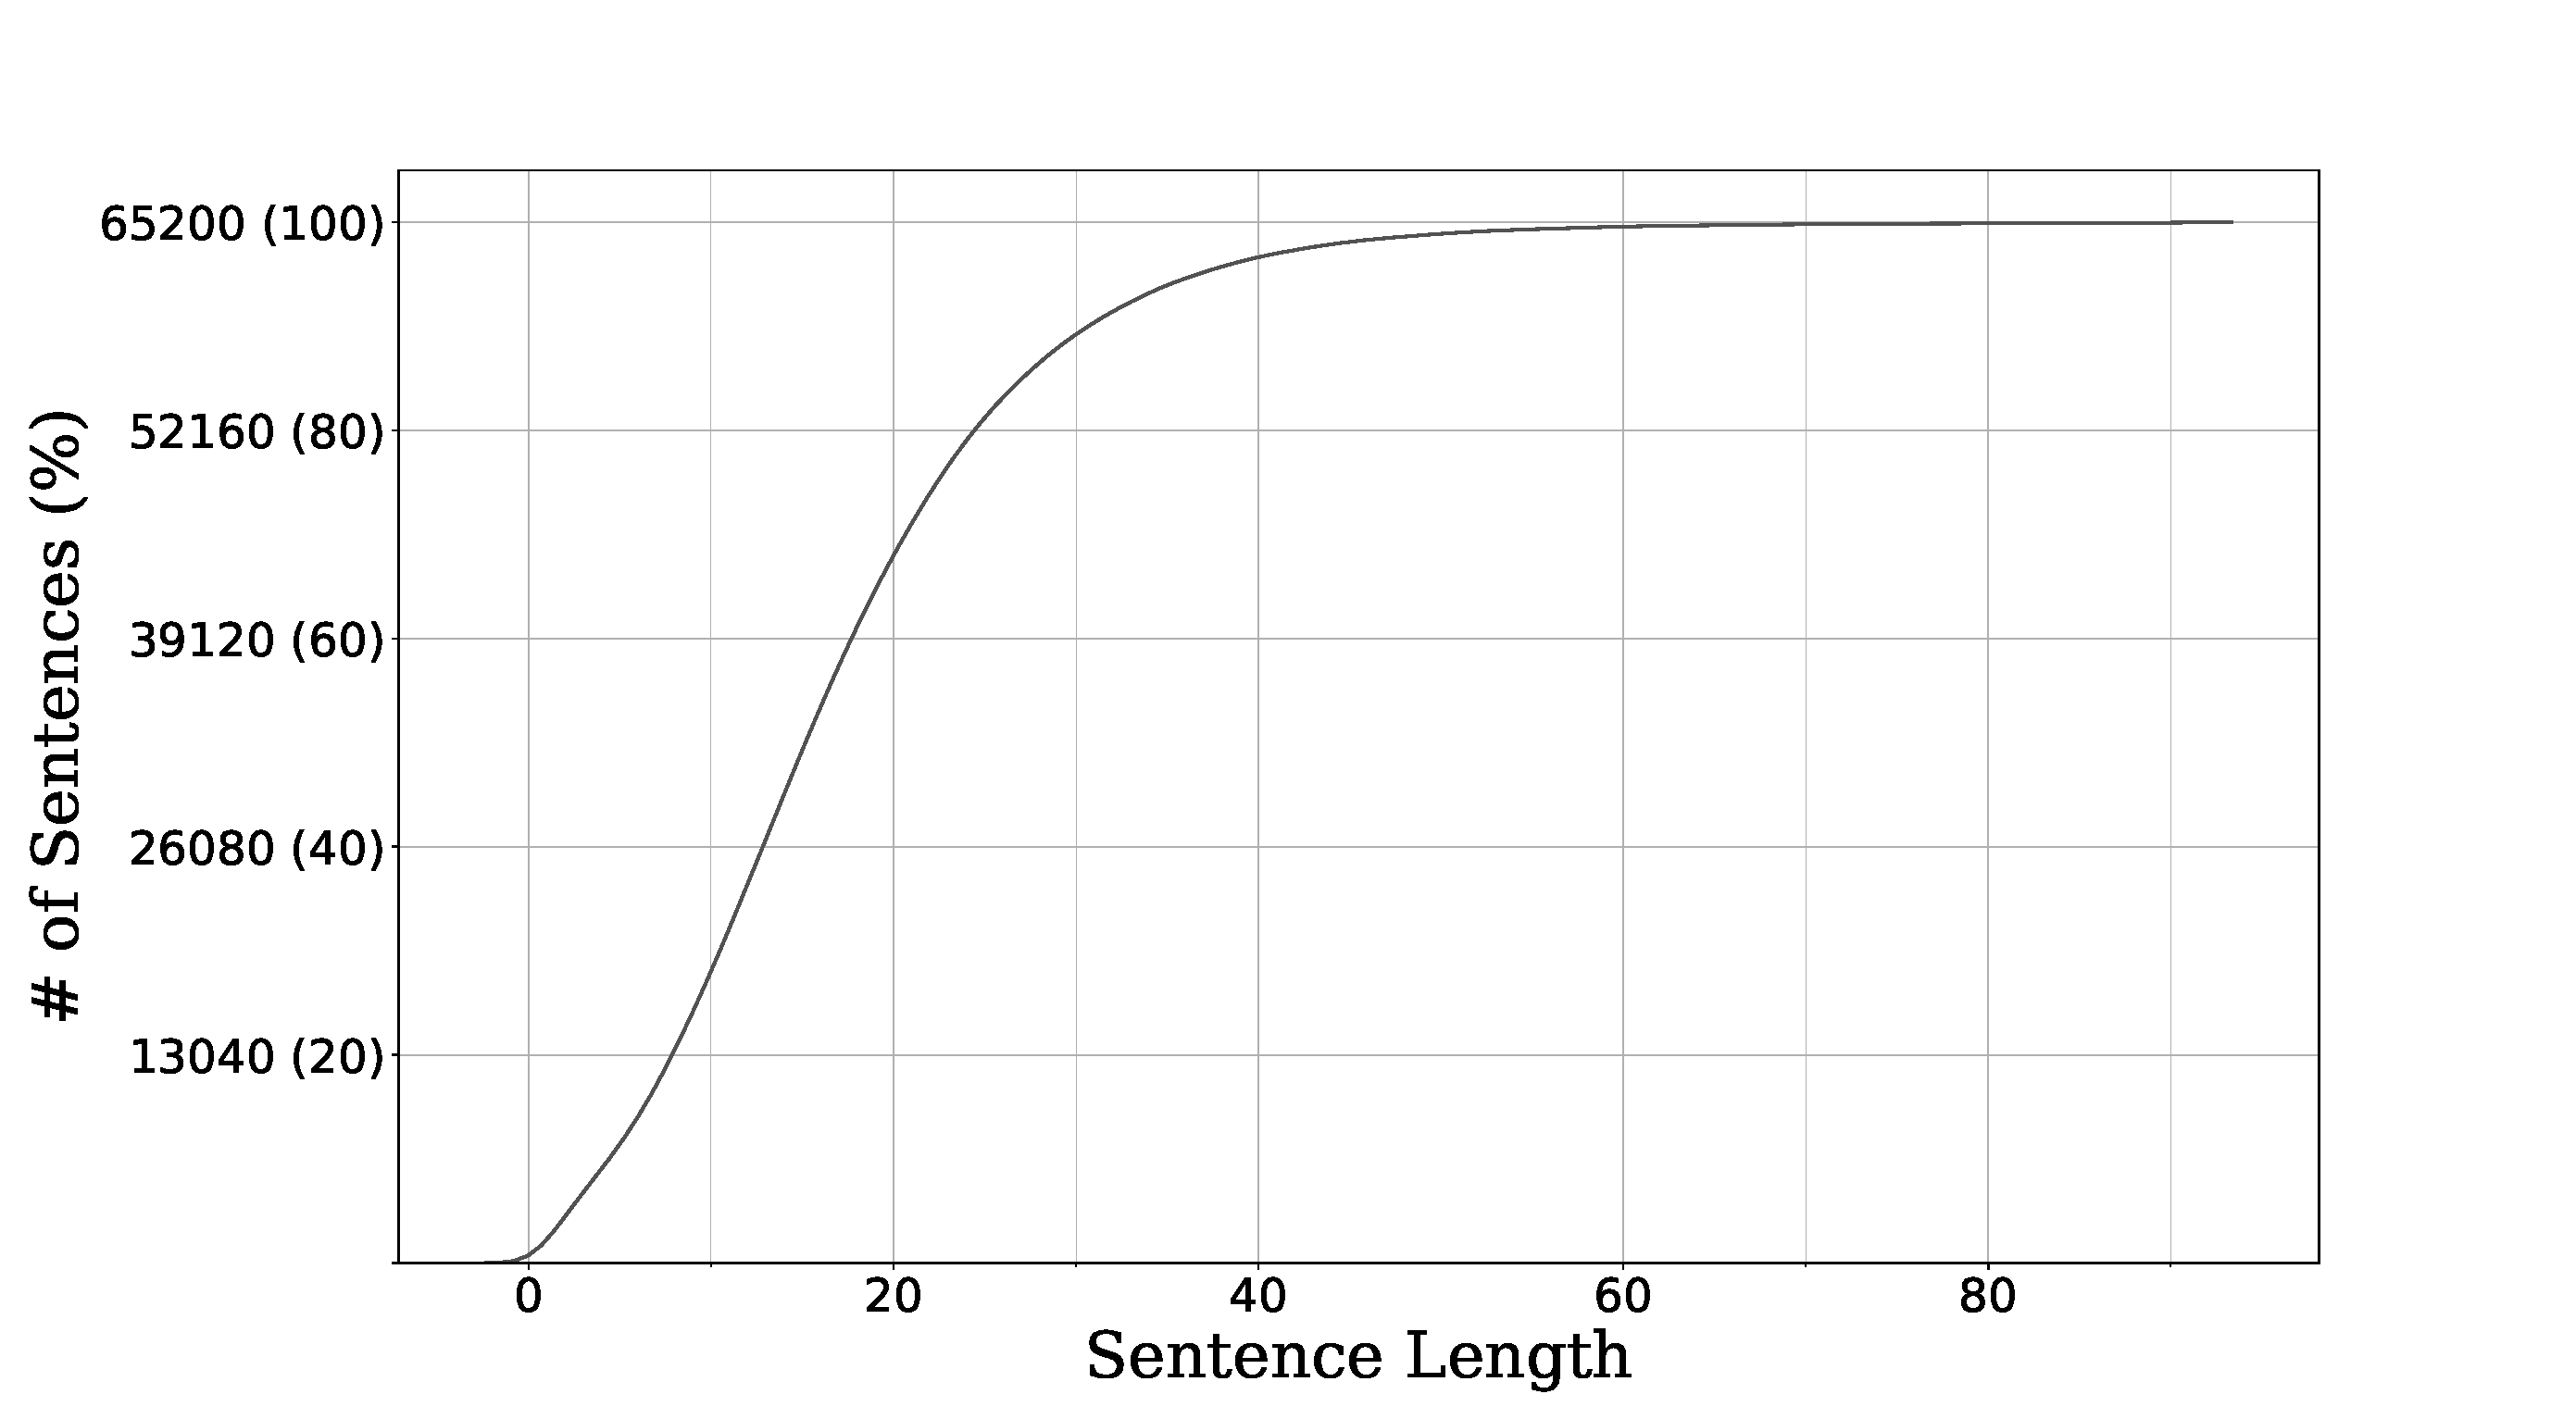
\includegraphics[scale=0.29]{Figures/len.pdf}
    \caption[Lassy-Small Sentence Lengths]{Cumulative sentence lengths in the original corpus, including punctuation.}
    \label{fig:lassy_sentence_lens}
\end{figure}

\section{Extraction Process}
% We can now move to describing the algorithmic framework designed for the extraction process.
% We will start with an exposition of the general algorithm, momentarily assuming full compatibility between the input and its internal routines.
% This compatibility is ensured through a means of pre-processing steps and added subroutines for exceptional case management, detailed immediately after the extraction's core is presented.

\subsection{Extraction Algorithm}
\label{subsec:extraction_alg}
Algorithms~\ref{alg:utils} and~\ref{alg:ra} summarize the type-assignment process, subdivided into components. 
The first revolves around utility functions that implement contextual assignment of phrasal arguments, root nodes and modifiers, as well as a method that concerns the binarization of multi-argument functors.
The second presents a method for iterating over a DAG.
During the iteration, the DAG's nodes are decorated with types by calling the prior functions as needed.
The goal here is to draw a rough sketch of the overall process rather than delve into a detailed description.
In that sense, the presentation abstracts away from the minutiae of the implementation, but also makes a few simplifying assumptions, namely the full compatibility between the system's routines and its input, as well as an absence of exceptional cases.
These simplifications will be easier to address after the extraction's core has been exposed.

\begin{algorithm}{
\caption{Type Assignment Utilities}\label{alg:utils}
\begin{algorithmic}[1]
\Procedure{Trans}{node $N$}\label{alg:ra:trans:start}\\
\Comment{Translates independent nodes to atomic types}
\If{is\_terminal($N$)}
    \State $\textbf{return}$ pos\_table[$N$.part\_of\_speech]
\Else
    \State $\textbf{return}$ cat\_table[$N$.syntactic\_category]
\EndIf
\EndProcedure\label{alg:ra:trans:end}
\\
\Procedure{TypeAssign}{node $N$, dependency $dep$, parent\_type $\textsc{p}$}\\
\Comment{Assigns contextually-informed types to modifiers and arguments}
\label{alg:ra:typeassign:start}
\If{$dep$ $\in$ mod\_labels}
    \State $d$ $\gets$ dep\_table[dep]
    \State $\textbf{return}$ $\textsc{p}\myrightarrow{d}\textsc{p}$
\Else
    \State $\textbf{return}$ $\textsc{Trans}(N)$
\EndIf
\EndProcedure
\label{alg:ra:typeassign:end}
\\
\Procedure{MakeComplex}{Arguments $A$, Result \textsc{r}}\\
\Comment{Converts a list of type \& dependency pairs and a result into a binarized functor}
\label{alg:ra:makecomplex:start}
    \State $A$ $\gets$ sort($A$)
    \State $D$ $\gets$ map(snd, $A$)
    \State $d_1, \dots, d_n$ $\gets$ map(dep\_table, $D$)
    \State \textbf{return} $\textsc{a}_1$ $\myrightarrow{$d_1$}$ $\textsc{a}_2$ \dots $\textsc{a}_N$ $\myrightarrow{$d_N$}$ \textsc{r}
    \label{alg:ra:makecomplex:fold}
\EndProcedure
\label{alg:ra:makecomplex:end}
\end{algorithmic}
}
\end{algorithm}

\paragraph{Arguments and Modifiers}
The simplest, primitive component is a function \textsc{Trans} (\ref{alg:ra:trans:start}-\ref{alg:ra:trans:end}).
It simply distinguishes between leaves and non-terminals, extracts the part-of-speech  or syntactic category tag respectively, and uses the corresponding translation table to map it to an atomic type.
The instantiation of the type translation tables is presented in Table~\ref{table:lex}.
\textsc{Trans} is a context-agnostic type-assignment function; it is used to assign direct phrasal dependents and root nodes, the typing of which depends neither on their ancestors nor their descendants.

Modifiers require different treatment; their types are instances of the parametrically polymorphic scheme:
\[
\textsc{t} \myrightarrow{d} \textsc{t}
\]
where \textsc{t} the type of the phrase being modified and $d$ the dependency label enacted by the modifier (an element of closed set).
In the current implementation, aside from plain modifiers (\textit{mod}), appositions (\textit{app}) and predicate modifiers (\textit{predm}) are also treated as modifying labels.
To correctly instantiate modifier types, we implement a minimally context-aware typing function, \textsc{TypeAssign} (\ref{alg:ra:typeassign:start}-\ref{alg:ra:typeassign:end}).
Given a node, the type of the node's parent and the dependency linking the two, it either assigns a type according to the above scheme, if the dependency is modifying, or defaults to \textsc{Trans} otherwise.
In the former case, the dependency is translated into an implication name through a translation table; its running instantiation is presented in Table~\ref{table:colors}.

\paragraph{Head Types}
At this point we need to recall that our complex types are unary functors, i.e. they have a single argument and produce a single result.
Yet the DAGs' branchings are not binary, and the pervasiveness of word-order freedom in the language means that a large degree of argument permutation is to be anticipated within multi-argument types.
Acknowledging these permutations is meaningful for parsing, but less so for semantic tasks; the order of words matters little if their dependencies are already specified.
Additionally, permitting multiple different representations for types that are functionally equal has the negative side-effect of enlarging the size of our extracted type lexicon.
As a counter-measure, we may enforce unary functor types by setting up an order over types, dictating their proximity to the end-result when they participate as arguments in the construction of a complex type.
Function \textsc{MakeComplex} (\ref{alg:ra:makecomplex:start}-\ref{alg:ra:makecomplex:end}) utilizes such an order, implemented as a sorting of a list of pairs of types \& dependencies.
The concrete implementation may remain unspecified for now; we will return to it at a later stage.
The main functionality is generally independent of the sorting criterion; the type-dependency pairs are sorted, and their dependencies are translated into implication names.
Then, a unary functor is built up by folding over the sequence in reverse order, using the result type as the initial argument and the next sequence item as the new outer argument (\ref{alg:ra:makecomplex:fold}).

\paragraph{Recursive Type Assignment}
Finally, the bulk of the work is carried out by \textsc{RecursiveAssignment} (\ref{alg:ra:recursiveassignment:start}-\ref{alg:ra:recursiveassignment:end}).
Given a parent node, its type, and a partially filled dictionary mapping nodes to types, it is responsible for carrying out the type-assignment for the part of the DAG that lies below.
First, it inspects whether the parent node is a leaf, in which case the current call terminates.
Otherwise, it inspects the node's daughters and their corresponding edges, and selects for the head (\ref{alg:ra:recursiveassignment:select_head}). 
Note that for this to work, a deterministic process for selecting a head is necessary; in other words, all structures are considered headed. 
Head-daughters can be told apart by their incoming dependency label, which is either of head (\textit{hd}), relative-clause head (\textit{rhd}), wh-clause head (\textit{whd}), comparative (\textit{comp}) or coordinator (\textit{crd}).
An empty list is then instantiated for arguments to be filled by type \& dependency pairs.
Next, the algorithm iterates over the node's daughters, deciding the type of each via \textsc{TypeAssign}.
For each daughter, an empty list of embedded arguments, also being type \& dependency pairs is also instantiated.
A full downwards iteration of the DAG, starting from that daughter is carried out.
If at any time a descendant node is identified with the current call's head, its type, as inferred by \textsc{TypeAssign} called with the new-found inner dependency and the current daughter as arguments, is added to the embedded argument list.
After this iteration is complete, the dependency between the daughter and the current parent node is inspected; if it bears no secondary marking, the type dictionary is updated and \textsc{RecursiveAssigment} is called anew on the daughter using its inferred type.
Recursive calls of this function essentially fill in types for the DAGs' elements in a depth-first, left-biased manner.

When the control returns to the caller function, the daughter's type is updated by applying \textsc{MakeComplex} using the embedded argument list and the previous daughter type.
If the embedded argument list is populated, one of the daughter's (not necessarily immediate) descendants is also its sibling.
The updated type then reflects the incomplete nature of the DAG rooted at this daughter, and the need for hypothetical reasoning to resolve the lexically immaterial arguments.
Finally, if the main dependency between the parent node and the daughter currently examined is not a modifier, the daughter's type is added into the argument list.

After all daughters have been processed, iterated through and their types assigned, the next step is to construct the head's type.
Since the embedded arguments already account for gaps, the head is simply functor from the argument types (as collected in the arguments list) to the parent's type.

It is now straightforward to annotate a full DAG by simply selecting its root node, finding its type via a direct translation, initializing an empty dictionary, and filling it via \textsc{RecursiveAssignment} which is simply called with the prior arguments (\ref{alg:ra:annotatedag:start}-\ref{alg:ra:annotatedag:end}).

\begin{algorithm}{
\caption{Type Assignment Process}\label{alg:ra}
\begin{algorithmic}[1]
\Procedure{RecursiveAssignment}{node $N$, node\_type \textsc{p}, type\_dict $\mathcal{D}$}\\
\Comment{Depth-first recursion over a partial DAG}
\label{alg:ra:recursiveassignment:start}
    \If{is\_terminal($N$)}
        \State $\textbf{exit}$
    \EndIf
    \State $head \gets$ select\_head($N$.daughters)
    \label{alg:ra:recursiveassignment:select_head}
    \State $arguments \gets []$
    \For{(daughter $d$, dependency $dep$) \textbf{in} $N$.daughters $\wedge$ \{head\}}
        \State $daughter\_type \gets$ \textsc{TypeAssign}($d$, $dep$, \textsc{p})
        \State $embedded\_args \gets$ []
        \label{alg:ra:recursiveassignment:findhot:start}
        \For{(descendant $f$, dependency $inner\_dep$) \textbf{in} $d$.descendants}
            \If{$f$ == head}
                \State $inner\_type \gets$ \textsc{TypeAssign}($f$, $inner\_dep$, daughter\_type)
                \State $embedded\_args$.append([$inner\_type$, $inner\_dep$])
            \EndIf
        \EndFor
        \label{alg:ra:recursiveassignment:findhot:end}
        \If{is\_primary($dep$)}
            \State $\mathcal{D}[d] \gets daughter\_type$
            \State \textsc{RecursiveAssignment}($d$, $daughter\_type$, $\mathcal{D}$)
        \EndIf
        \State $daughter\_type \gets$ \textsc{MakeComplex}($embedded\_args$, $daughter\_type$)
        \If{$dep$ $\notin$ mod\_labels}
            \State $arguments$.append([$daughter\_type$ $\otimes$ $dep$])
        \EndIf
    \EndFor
    \State $\mathcal{D}$[$head$] $\gets$ \textsc{MakeComplex}($arguments$, \textsc{p})
\EndProcedure
\label{alg:ra:recursiveassignment:end}
\\
\Procedure{AnnotateDAG}{DAG $G$}\\
\Comment{Type annotates a full parse DAG}
\label{alg:ra:annotatedag:start}
    \State $r$ $\gets$ $G$.root
    \State $\mathcal{D}$ $\gets$ \{\}
    \State \textsc{t} $\gets$ \textsc{Trans}($r$)
    \State \textsc{RecursiveAssignment}($r$, \textsc{t}, $\mathcal{D}$)
    \State \textbf{return} $\mathcal{D}$
\EndProcedure
\label{alg:ra:annotatedag:end}
\end{algorithmic}
}
\end{algorithm}

\paragraph{Argument Ordering}
To consistently binarize multi-argument complex types, we establish a strict partial order over the set of dependency relations.
The order is motivated by the obliqueness hierarchy present within verbal arguments, loosely inspired by~\cite{dowty}\footnote{Even though this ordering is normally established relative to the result category, we can simplify the process by considering that incompatible arguments will not compete for hierarchy within a single functor --- thus, no more than one partial order is necessary.}.
The sorting algorithm then arranges a sequence of type \& dependency pairs based solely on the latter.
Figure~\ref{fig:lattice} depicts the Hasse diagram of the poset, where incomparable items are collapsed into a single set.
These either never co-exist as arguments to the same functor due to being subclasses of the same dependency (such the various instances of clause bodies) or occupying mutually exclusive positions (as in the complemental verbal arguments), or when they do their order is irrelevant (e.g. modifiers).
In the case of incomparable items appearing simultaneously, an alphabetical default is applied.
Even though conjuncts and modifiers do not directly belong in the obliqueness hierarchy, they are positioned in the poset in a way that ensures type readability and sanity; for instance, modifiers are always placed last, so if a functor corresponds to a modifier construction, the resulting modifier type will always appear last.
Similarly, coordinators are not derived but may still partake in higher-order types; as such, conjunction dependencies always appear first.

\begin{figure}
\centering
\begin{tikzpicture}
\matrix (a) [matrix of nodes, column sep=0.5cm, row sep=0.6cm]{
\{cnj\} \\
\{invdet\} \\
\{su\} \\
\{pobj\} \\
\{obj1\} \\
\{predc, obj2, se, pc, hdf\} \\
\{ld, me, vc\} \\
\{svp\} \\
\{whd\_body, rhd\_body, body\}\\
\{app, predm, mod\}\\
};

\draw (a-1-1) -- (a-2-1) ;
\draw (a-2-1) -- (a-3-1);
\draw (a-3-1) -- (a-4-1);
\draw (a-4-1) -- (a-5-1);
\draw (a-5-1) -- (a-6-1);
\draw (a-6-1) -- (a-7-1);
\draw (a-7-1) -- (a-8-1);
\draw (a-8-1) -- (a-9-1);
\draw (a-9-1) -- (a-10-1);

\end{tikzpicture}
    \caption[Dependency Role Obliqueness Ordering]{Dependency role obliqueness ordering. Lower roles take precedence in priority over higher ones (appear closer to the result)}
    \label{fig:lattice}
\end{figure}


\subsection{Transformations and Exceptions}
\label{subsec:transformations}

The extraction algorithm, as specified earlier, makes a few assumptions pertaining to the DAGs' structure, which are not always valid.
In order to bring the corpus to a format that is maximally compatible with the algorithm, a series of preprocessing steps, in the form of conversions of the original annotation, become necessary.
In addition, on several occasions correct type inference requires a few alterations to the general algorithm flow, implemented in the form of conditional case management.
The paragraphs below detail these transformations and exceptions.
For most transformations a visual example is provided, depicting the derivation's DAG before and after its application.

\paragraph{From Trees to DAGs}
To begin with, ``phantom'' nodes are useful for maintaining a tree-like view of the DAG, but are otherwise hard to utilize.
In only being linked to a subset of the lexical item's ancestors, they obfuscate the overall parse structure, necessitating multiple iterations to distinguish and type-assign.
For that reason, we remove node copies by allowing multiple incoming edges onto a single node.
To distinguish between edges provided by the original treebank and edges inserted by the transformation, we refer to the former as primary and the latter as secondary.
Any non-root node is always associated with exactly one incoming primary edge, and zero or more secondary edges.
This invertible transformation serves mostly representational and algorithmic needs, in the sense that it permits us to refer to a node as a single unit regardless of the multiplicity of roles it assumes within the parse structure. 

\paragraph{Abstact Semantic Arguments}
Lassy's annotation scheme includes secondary edges for verbs' abstract semantic arguments embedded under past participial phrases and infinitival clauses.
These dependencies account for semantic flows within sentences, but in doing so escape from the boundaries imposed by the phrase-local syntax.
Furthermore, the distinction between primary and secondary edge labeling in the case of abstract arguments is not structurally consistent, injecting a source of unnecessary ambiguity for the type extraction.
In light of the above, we first homogenize the labeling by setting the node that resides at the higher level of the graph as the primary one in all ambiguous constructions.
Since embedded clauses are systematically dependents of primary clauses, this may be viewed as equating between sentence-primary roles and primary edges.
We can then consistently remove all abstract arguments by simply filtering out secondary links with a subject or object label that occur between past participles/infinitives and their daughters, if the latter have a primary subject or object link with an (immediate or otherwise) ancestor of their direct parents.
An example of the transformation is presented in Figure~\ref{fig:abstract_arg}.

\begin{figure}[t]
    \begin{subfigure}[t]{0.49\textwidth}
        \centering
        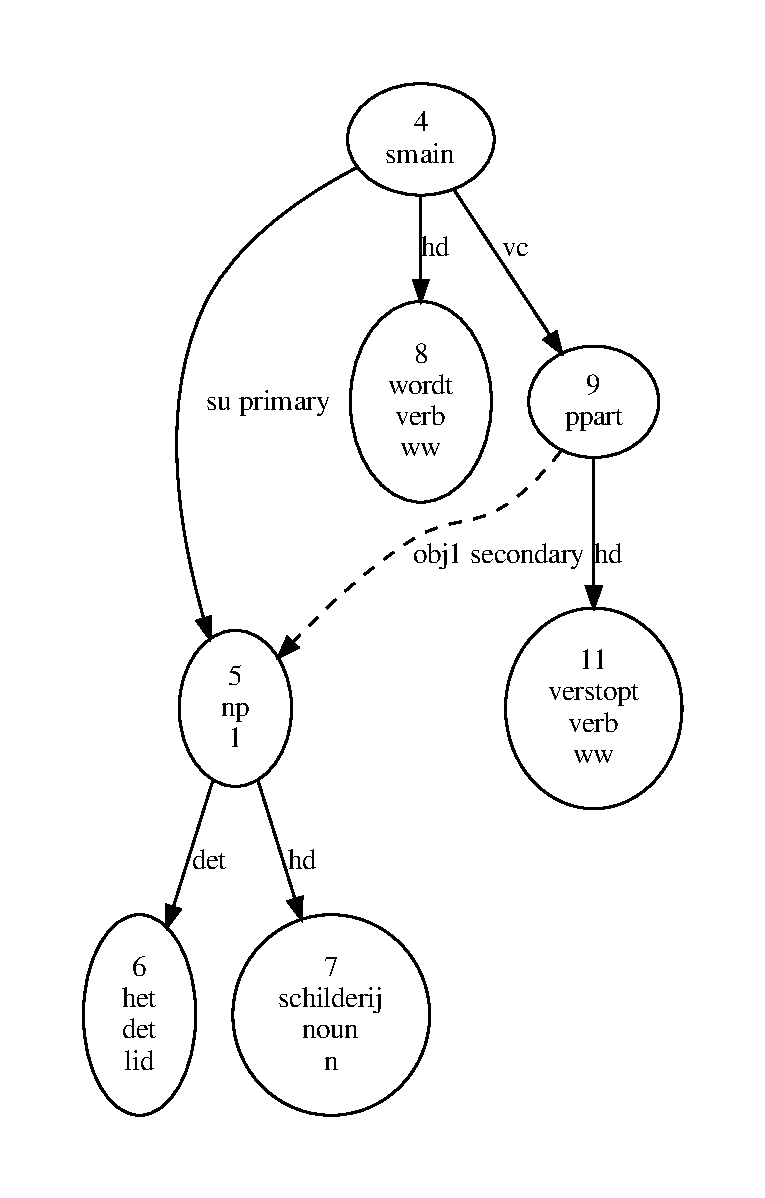
\includegraphics[scale=0.49]{Figures/abs1.pdf}
        \caption{Before removal}
        \end{subfigure}
    \begin{subfigure}[t]{0.49\textwidth}
        \centering
        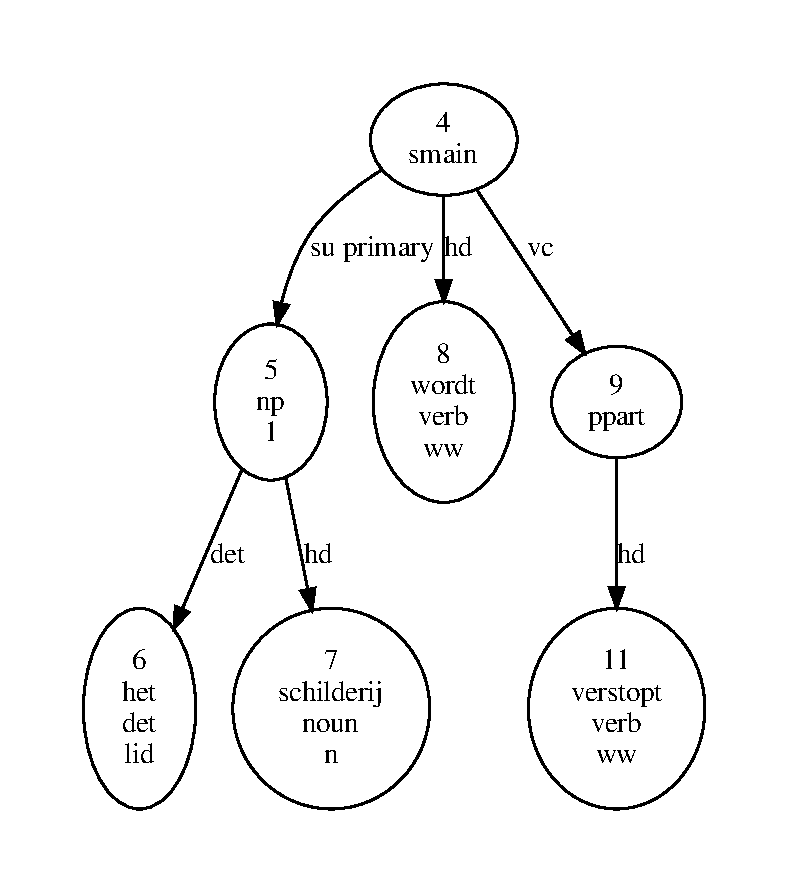
\includegraphics[scale=0.49]{Figures/abs2.pdf}
        \caption{After removal}
    \end{subfigure}\vfill
    \caption[Abstract Semantic Argument Removal]{Derivation structure before (a) and after (b) abstract semantic argument removal for the sentence ``het schilderij wordt verstopt'' (\textit{The painting was hidden}). The phrase ``het schilderij'' acts as both a subject argument for the main sentence verb ``is'' and the understood object for the participial head ``verstopt''. After the transformation, the second dependency is erased.}
    \label{fig:abstract_arg}
\end{figure}

\paragraph{Noun-Phrase Headedness}
When determiners and nouns are participating in the formation of a phrase, nouns are assigned the head-role to which determiners act as dependents.
Without making any argument for determiner-headed phrases, we acknowledge two problems with treating nouns as functors.

First, for the type grammar itself, it would mean that nouns are contextually-typed --- a noun in isolation might act as an independent noun-phrase, whereas a noun paired with a determiner is a functor type from determiners to noun-phrases.
Secondarily, anticipating a future semantic interpretation of our type system, we would like nouns to be viewed as atomic, individual objects rather than functions, for reasons both practical and conceptual.
To avoid the linguistic repercussions of considering determiners as heads, we opt to make a distinction between headedness and functoriality in this particular case.
Treating determiners as the phrasal functors resolves both of the above problems, as they consistently appear paired to a nominal (which may be seen as their argument), and can be trivially interpreted into identity maps in the semantic space (thus preserving the content of their arguments).

For these reasons, we choose to alter the dependency labels internal to noun-phrases as follows; determiner labels are set to head labels (for compatibility purposes) and head labels occupied by nouns are set to a dual of the determiner, which we name \textit{invdet}.
An example of the transformation is shown in Figure~\ref{fig:invdet}.

\begin{figure}[t]
    \begin{subfigure}{0.49\textwidth}
        \centering
        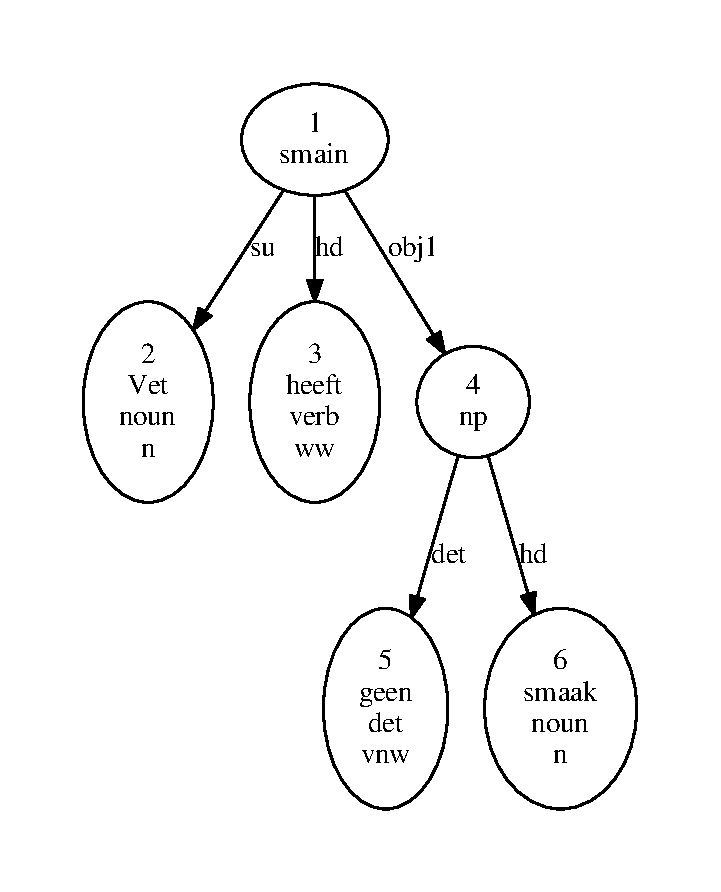
\includegraphics[scale=0.48]{Figures/invdet1.pdf}
        \caption{Before swapping}
    \end{subfigure}
    \begin{subfigure}{0.49\textwidth}
        \centering
        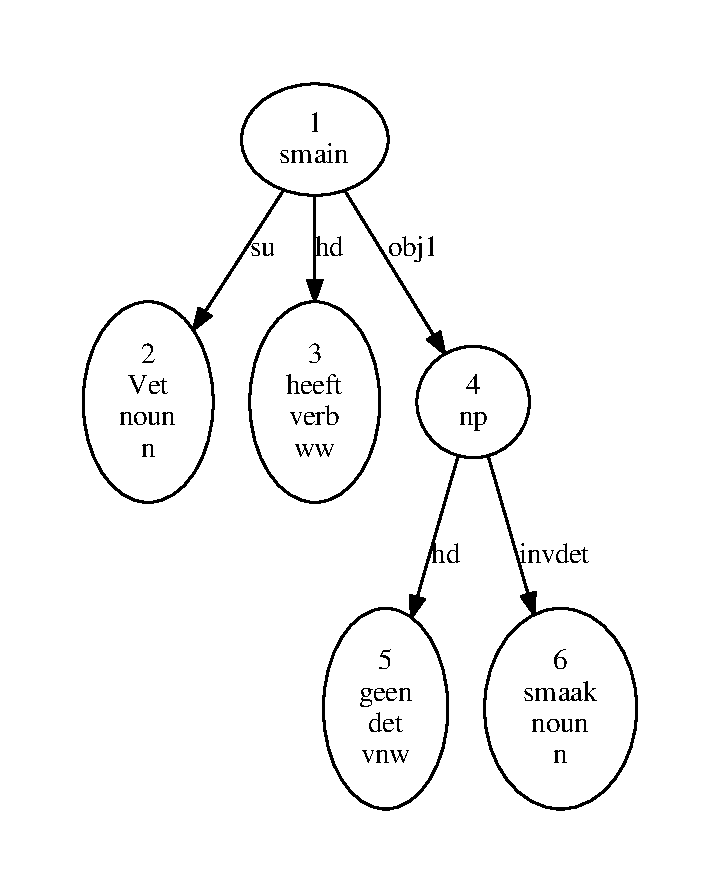
\includegraphics[scale=0.48]{Figures/invdet2.pdf}
        \caption{After swapping}
    \end{subfigure}
    \caption[Noun-Phrase Head Swapping]{Dependency relation naming before (a) and after (b) swapping noun-phrase heads for the example sentence ``Vet heeft geen smaak' (\textit{Fat has no taste}). The pronoun ``geen'' acts as a determiner to the noun-phrase ``geen smaak''. After the transformation, it is assigned the head role, with the noun-phrase being assigned the dual label \textit{invdet}.}
    \label{fig:invdet}
\end{figure}

\paragraph{Numerals and Multiple Determiners}
The transformation described above is not always as straightforward.
Although it is the case that each noun-phrase has a single head-noun, it is not the case that it has a single determiner.
The most common instance of a noun-phrase with more than one determiner are phrases that contain numerals and count-words, the dependencies of which are also labeled as determiners.
Examples of such phrases include ``de twaalf profeten'' (\textit{the twelve prophets}), ``de beide zijluiken'' (\textit{the two side-panels}) etc. 
These cases are easy to solve by simply adjusting the numerals' dependency label into modifier (\textit{mod}), when they co-exist with a real determiner.
If a numeral is the sole companion of a nominal, we allow it to retain its determiner role, meaning it later gets converted into the phrasal functor.
An example of the transformation is depicted in Figure~\ref{fig:tw_to_mod}.

A less frequent but more problematic instance is that of determiner pairs, i.e. words that jointly form a determiner when occurring one next to the other, such as for example ``geen enkele'' (\textit{not a single one}), ``een enkele'' (\textit{one}), etc.
As hierarchy is not present on such expressions (no word dominates the phrase over the other), it is ill-advised to insert makeshift structure in the form of a binary branching determiner phrase.
To bypass this issue, we set the first item's label to head, and assign a placeholder label \textit{\_det} to the second one. 
During the type assignment process, leaves carrying the special label default to the \textsc{\_det} type, to be read as \textit{second item of a determiner pair}. 
Functionally, it is as a marking above the logical language, denoting that this word needs to be collapsed with its immediately proximal neighbour to the left, forming a multi-word phrase that inherits the neighbour's type.


\begin{figure}[t]
    \begin{subfigure}{0.49\textwidth}
        \centering
        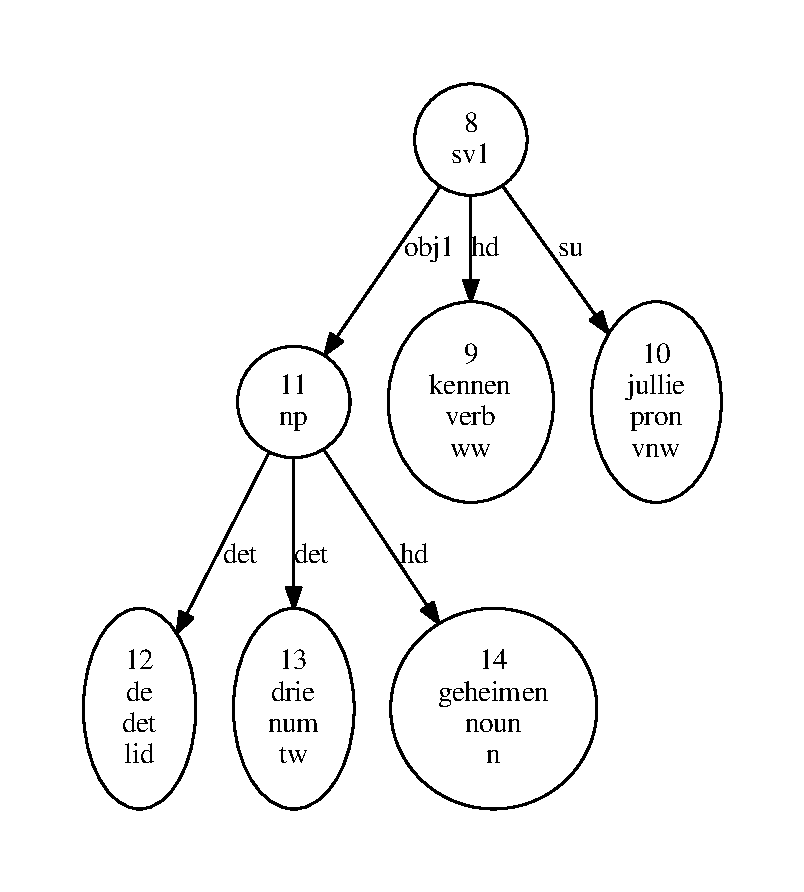
\includegraphics[scale=0.48]{Figures/tw_to_mod1.pdf}
        \caption{Before renaming}
    \end{subfigure}
    \begin{subfigure}{0.49\textwidth}
        \centering
        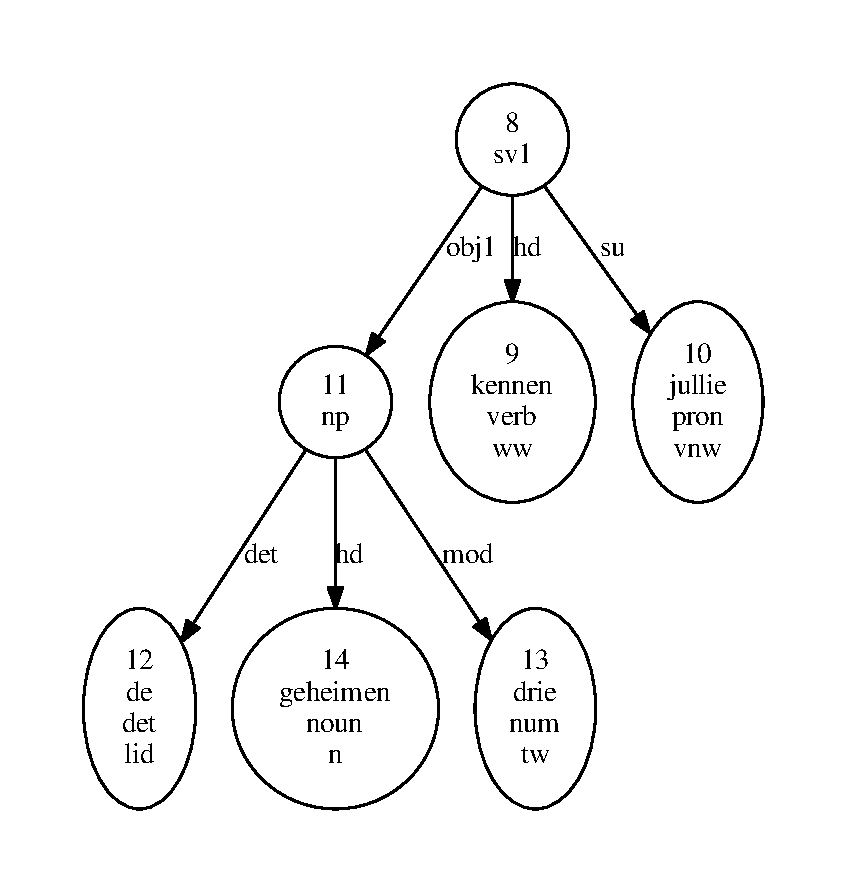
\includegraphics[scale=0.48]{Figures/tw_to_mod2.pdf}
        \caption{After renaming}
    \end{subfigure}
    \caption[Numeral Determiner Relabeling]{Dependency relation naming before (a) and after (b) the transformation of numeral determiners into modifiers for the example sentence ``kennen jullie de drie geheimen'' (\textit{do you know the three secrets}). Before the renaming, the numeral ``drie'' acts as an additional determiner for the noun-phrase ``de drie geheimen''. After the transformation, its dependency is altered to a modifier.}
    \label{fig:tw_to_mod}
\end{figure}

\paragraph{Head-Body Pairs}
A common construction in Lassy-Small is that of head-body pairs, which is used to annotate relative clauses, wh-questions and phrases, complementizers and comparisons.
To distinguish between the above, the head label is subclassed into three different instances; \textit{rhd} (for relative clause heads), \textit{whd} (for wh-question- and phrase-heads) and \textit{hd} (for all remaining scenarios).
Seeing as head labels do not come out in the type system (being that these are indicators of functoriality rather than refinements of implications), we transfer the refinement from the heads onto their respective body labels, replacing \textit{body} with \textit{rhd\_body} or \textit{whd\_body} according to the context.

\paragraph{Unheaded and Multi-Headed Structures}
An operational assumption for the algorithm is that all complex phrases have exactly one head.
This assumption is not a product of the algorithm's design, but rather the distinguishing feature of phrase structure grammars, and the driving force behind compositionality in the case of categorial grammars.
Lassy's annotation scheme abides by a dependency-based formalism; that means that not all of the analyses satisfy this assumption.
The problem is manifested in two distinct ways; in unheaded structures, i.e. branchings where no clear distinction between functor and argument(s) can be made between a node's daughters, and multi-headed structures, i.e. branchings where more than one head candidates co-exist.

Examples of the first include multi-word phrases, conjunctions and discourse-level annotations.
Multi-headed structures occur indirectly in the context of determiner pairs as described earlier, but also directly in coordinator pairing and discourse-level annotations.
As no universal, algorithmic solution can be designed to account for all incompatible analyses, the following paragraphs are concerned with specific solutions targeted at particular problematic instances.

\subparagraph{Multi-Word Phrases}
The original annotation usually refrains from specifying the structure of multi-word phrases, but not consistently.
Multi-word phrases are for the most part depicted as a node with the syntactic category tag \textit{mwu} (for multi-word unit), all daughters of which are leaves with their edges marked as \textit{mwp}.
This approach detracts from the quality of the types that could be assigned in two ways; first and foremost, the absence of specified functor-argument relations in combination with the lack of an algorithmic way to construct them disallows us from providing precise types at the word level.
Furthermore, the category label of \textsc{mwp} corrupts type assignments for words and phrases outside the multi-word phrase, whenever it partakes as an argument to the formation of wider phrases.

To treat the first problem, we opt for the least drastic solution; multi-word phrases are collapsed into a single node, their outgoing edges are cut-off, and their corresponding lexical item becomes a contiguous span of the sentence rather than discrete items of it. 
The purpose of this transformation is to simply hide the uninformative edges.
In practical terms, no real information is erased (seeing as the edges may be re-introduced at any point with no extra knowledge).
The impact of this transformation on later applications (e.g. supertagging) is also relatively minor; all it requires is an extra component that identifies multi-word phrases and collapses them into a single element to be later used by the type-assignment process, which can be implemented as a chunking algorithm.

To avoid explicitly defining a type for multi-word phrases (thus also the consequences of such a type), we implement \textit{majority voting scheme} with biased priorities that consistently converts the \textit{mwu} tag onto other tags.
The scheme relies on a simple but intuitive and general rule; the syntactic category of the multi-word phrase may be almost perfectly inferred by the categories of its daughters. 
Therefore, we simply sum the occurrences of each part-of-speech tag exhibited by its daughters. 
Most of the time, the set of these tags is singular, containing either the noun (\textit{n}) or the special (\textit{spec}) tag as its sole item, the latter being used as a catch-all tag.
If at least one of the above tags is present (possibly accompanied by a number of adjective sisters), we simply promote the multi-word unit to the noun phrase category.
Otherwise, if there is a significant difference between the occurrence ratios between tag pairs, we promote the major tag to its corresponding phrasal category. 
An example of the transformation is presented in Figure~\ref{fig:mwu}.

\begin{figure}[t]
    \begin{subfigure}[t]{0.49\textwidth}
        \centering
        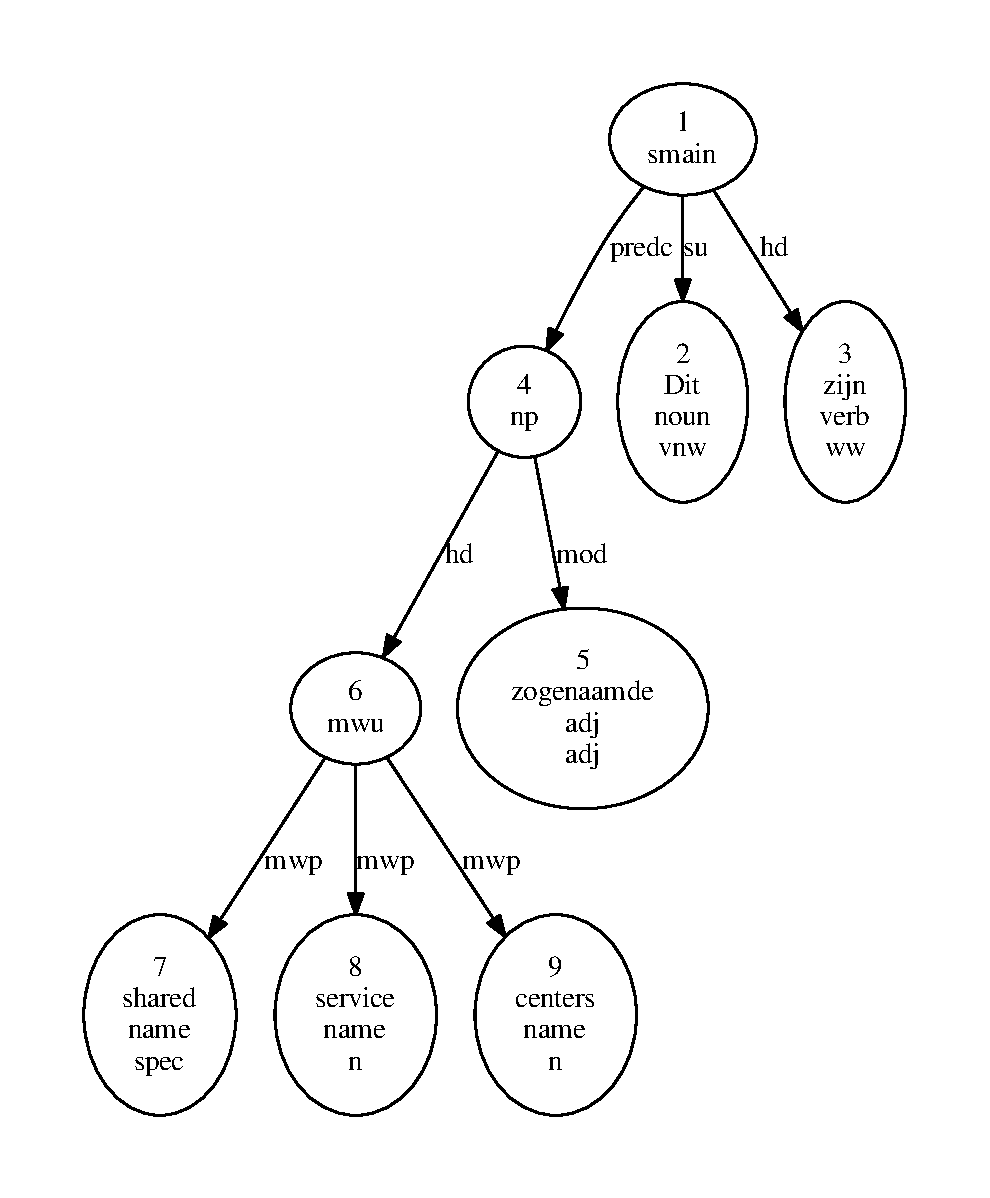
\includegraphics[scale=0.43]{Figures/mwu1.pdf}
        \caption{Before collapse}
    \end{subfigure}
    \begin{subfigure}[t]{0.43\textwidth}
        \centering
        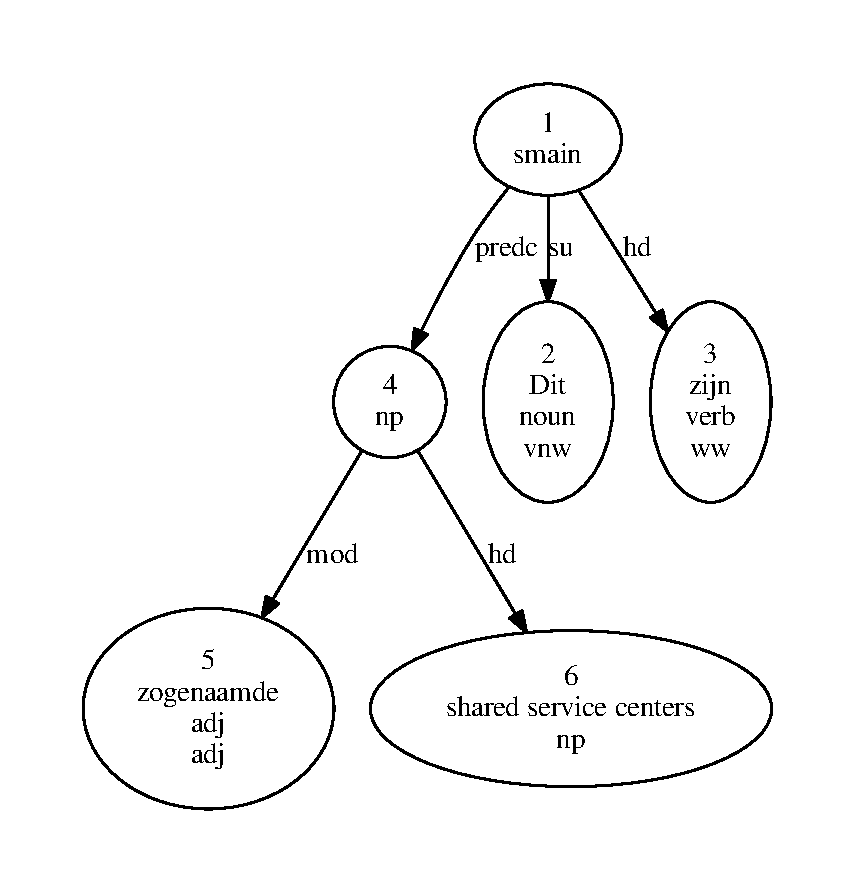
\includegraphics[scale=0.48]{Figures/mwu2.pdf}
        \caption{After collapse}
    \end{subfigure}
    \caption[Multi-Word Unit Collapse]{Derivation structure before (a) and after (b) the collapse of a mwu sub-DAG into a single for the example sentence ``Dit zijn zogenaamde shared service centers'' (\textit{These are so-called shared service centers}). Prior to the transformation, the phrase ``shared service centers'' is annotated as a sequence of nodes, rooted to a common ancestor. After the transformation, the three nodes are chunked into a single node that spans all three lexical items. The phrasal category of the new node is inferred by majority voting over its original children.}
    \label{fig:mwu}
\end{figure}

\subparagraph{Conjunction Phrases}
Conjunction annotations may pose problems in three different ways.

Quite like multi-word phrases, conjunction nodes are always assigned the syntactic category tag \textit{conj}, which is uninformative with respect to the conjunction's role or its contents.
The solution prescribed earlier in the form of a majority voting scheme is applicable in this case as well, modulo a minor difference.
Conjunctions are more general than multi-word units, in the sense that their constituents may carry a wider variety of tags.
When multiple daughter categories exist and their occurrence counts match, the decision on what tag to assign is not clear-cut; to account for conjunctions of uneven parts, we therefore expand upon the scheme by adding further biases.
The most informed decision we can make is to insert a preferential treatment towards sentential types, followed by nouns (assuming that all non-noun daughters are nominalized), followed by adjectives (assuming that participial phrases are used as adjectival phrases).
If neither of these preferences are satisfied, we default to the first item of the most highly occurring tag in the phrase.
We find this heuristic to be adequately performing; the uncertainty introduced when it is not is a minimal compromise.

Just like determiner pairs, conjunctions are sometimes coordinated not by a single head, but rather a pair of coordinators; for instance ``zowel.. als'' (\textit{such.. as}), ``respectievelijk ..en'' (\textit{respectively.. and}), etc. 
These pairs are again treated via a special type, \textsc{\_crd}, read as \textit{second item of a coordinator pair}, which looks for a coordinator type to its left (not necessarily adjacent) and collapses with it inheriting its type.

Finally, a major issue arises when a conjunction is unheaded.
This is a by-product of the annotation philosophy, which abstains from analyzing punctuation symbols, pushing them to the top of the parse with a default dependency under the root node.
Then conjunctions coordinated by comma(s) appear as simply an arrangement of sisters with no common head.
This lack of internal structure is not as easy to circumvent as in multi-word units.
Conjunction phrases can not be collapsed into a single item, as their daughters are not  necessarily leaves; they may be phrasal nodes, themselves containing a lot of important structure that cannot be ignored.
A considered solution would be to arbitrarily assign the head role to the first conjunct; this, however, would have the effect of potentially introducing exceedingly high-order functors to describe words further down the DAG, which bare little semblance to their actual phrase-local syntactic functionality.
The hard decision to make then is whether to enforce well-typedness at the sentence-level, or constrain the type scope to the local, conjunct-internal context, favoring corpus-wide uniformity and type clarity.
For the time being, we opt for the latter, leaving these constructions unheaded.
A temporary but minimally pervasive treatment for such analyses is detailed in the paragraph to follow. 
A future solution would be to attempt to push punctuation into the DAG and allow it to partake in or interact with the type assignment, filling in the gaps left by the missing coordinators.

\subparagraph{Discourse Labels and Headless Conjuncts}
Excluding multi-word phrases (for which an adequate solution has been realized), unheaded analyses amount to about 3\% of the overall branchings in the corpus.
These mostly include discourse-level annotations (nuclei, satellites, discourse links and parts), but also the aforementioned conjunctions with no coordinator.
The overall percentage is minor, but cannot be taken lightly; sentences containing at least one such branching occupy a non-negligible part of the treebank, and ignoring them would incur a significant loss of samples for the extraction and its later applications.
Given our inability to perform type inference in such scenarios, a solution that minimizes the sample loss is to instead split each unheaded branch, discarding problematic dependencies and all components above them, and treating each disjoint sub-DAG underneath as a new, independent phrase, rooted at the cut-off daughter node.
This way, we may still utilize proper annotations that are enclosed within unheaded structures under broader phrases.
The partial nature of the resulting DAGs remains in line with the rest of the treebank, as a number of unprocessed samples already portray phrases that do not stand as independent linguistic units.
The result of the splitting process is a new treebank which contains more but smaller samples; Figure~\ref{fig:dataset_lens} depicts the size and length distribution of the altered treebank.
The impact of this transformation is a decrease in the average length of a phrase of about 3 words (also including the removal of punctuations), and an increase in the corpus size by 3\,000 samples.

\begin{figure}
    \centering
    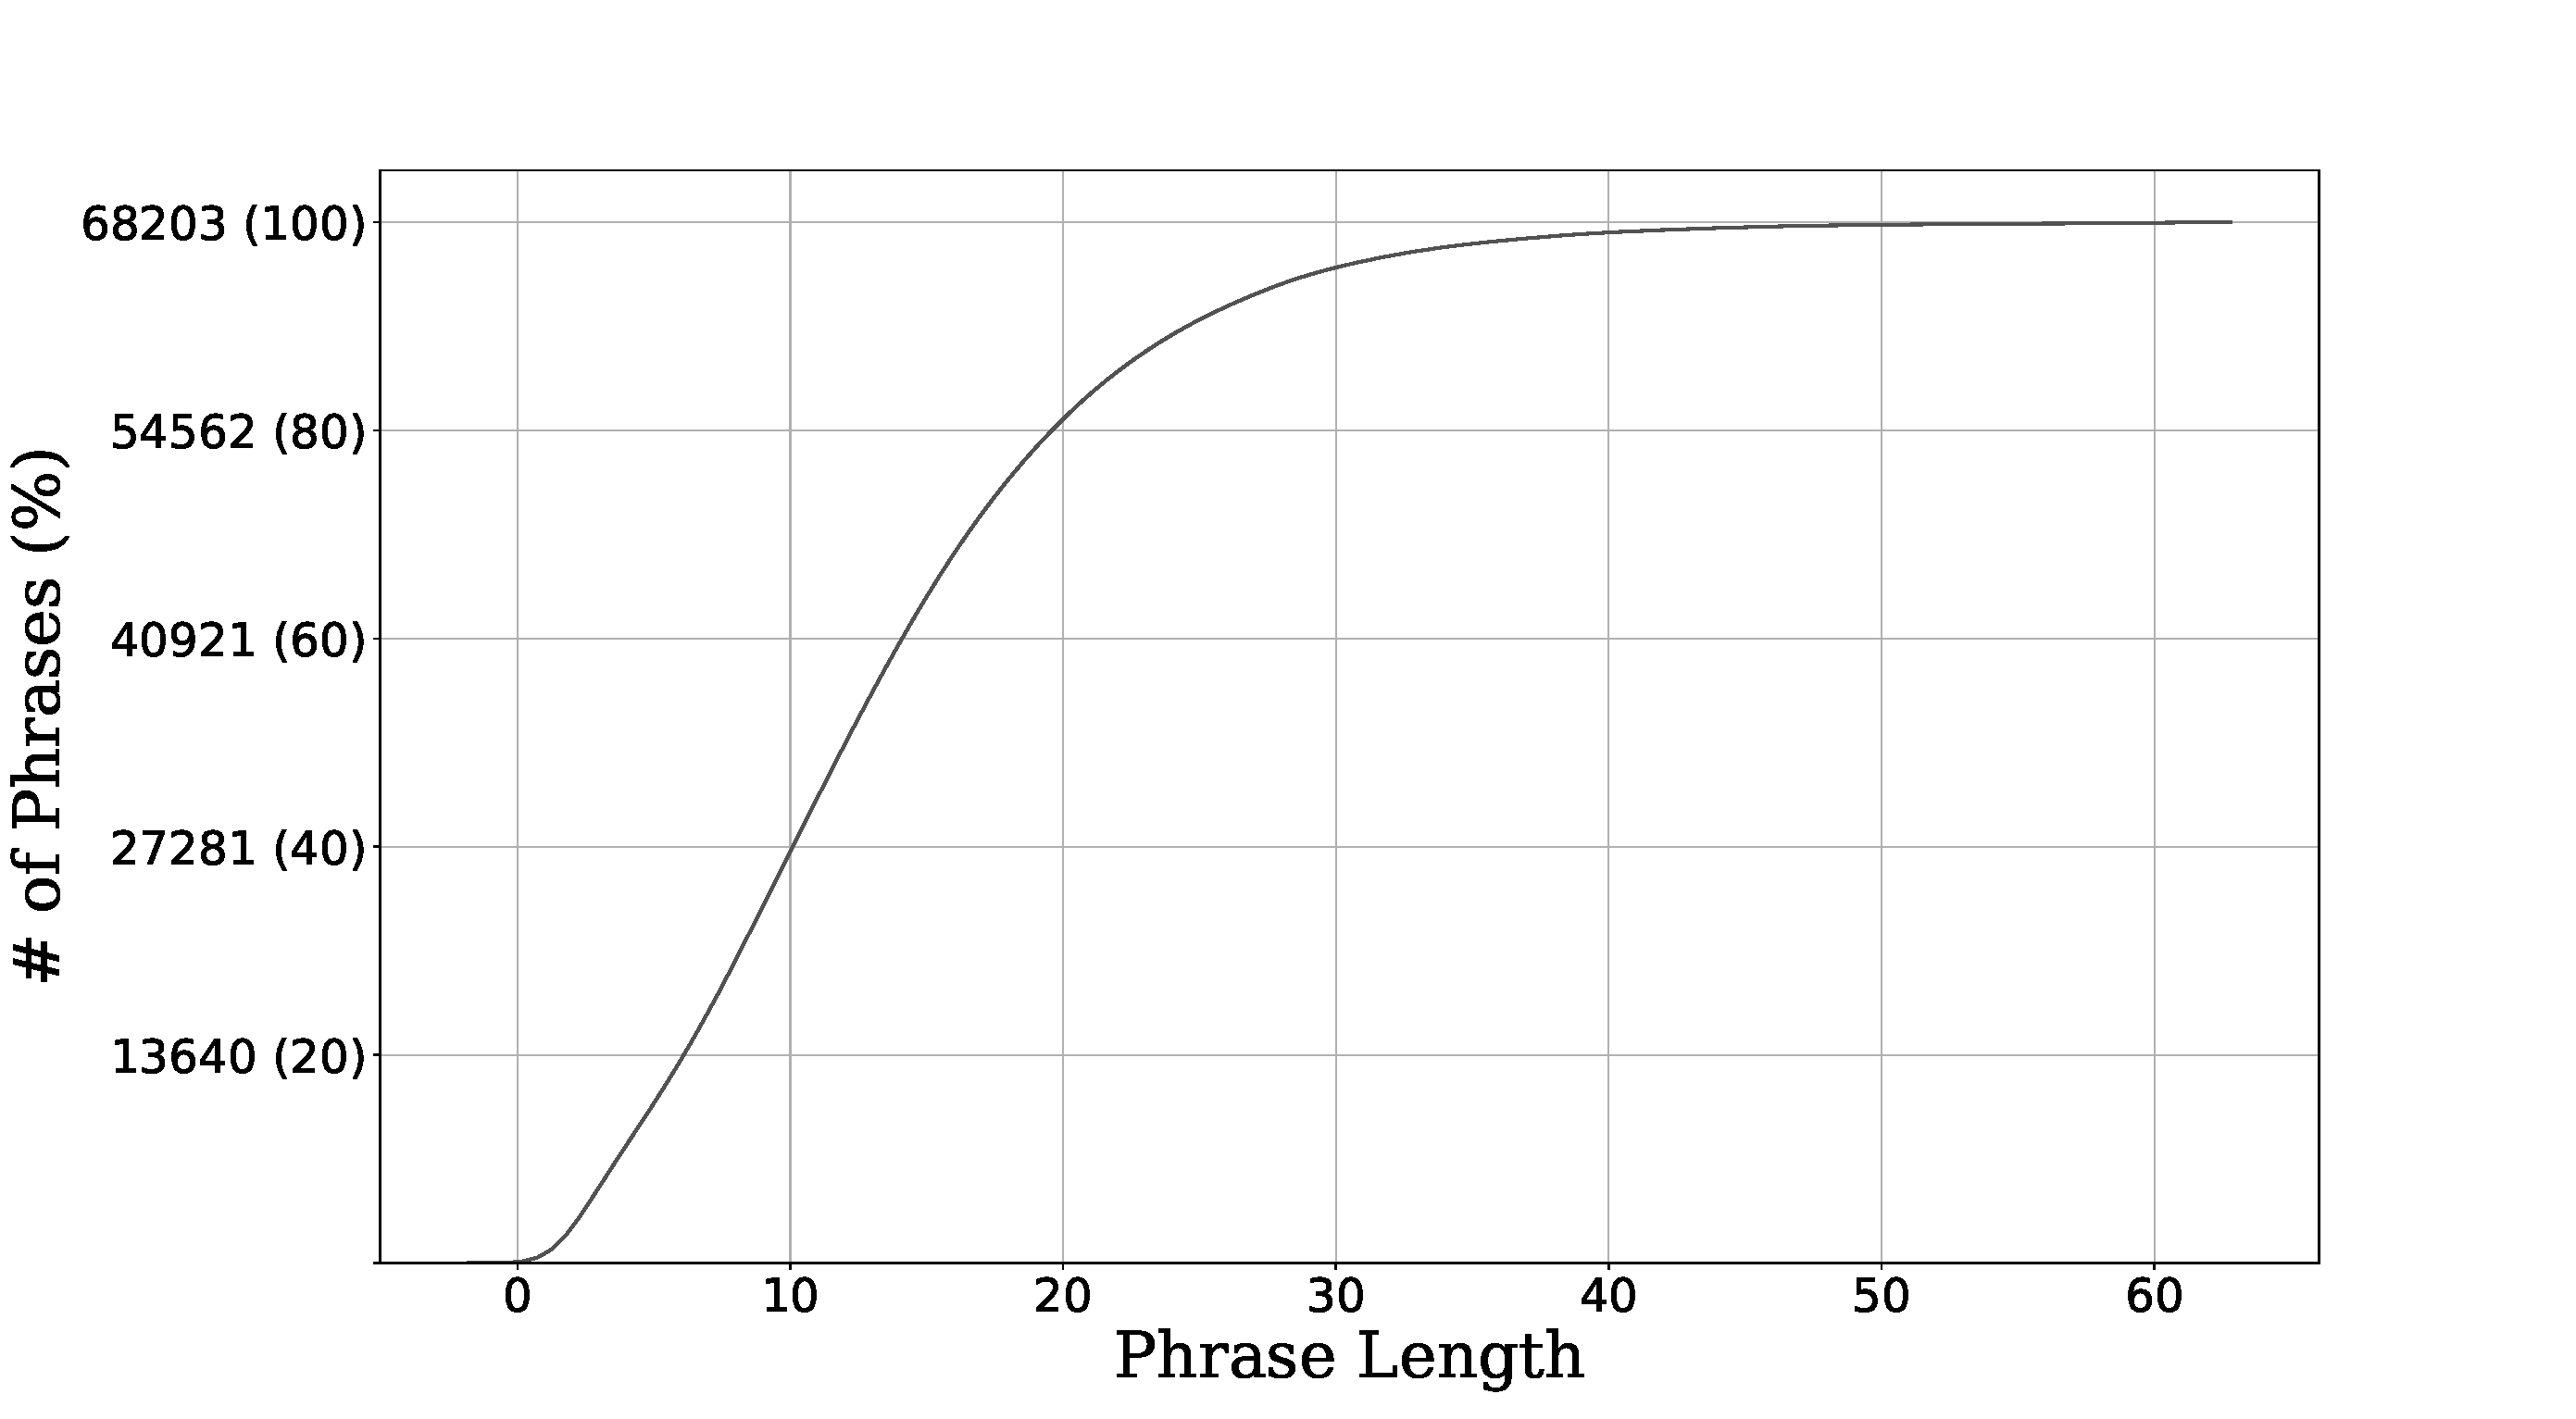
\includegraphics[scale=0.29]{Figures/lens2.pdf}
    \caption[Processed Phrase Sentence Lengths]{Cumulative phrase length in the processed corpus, excluding punctuation.}
    \label{fig:dataset_lens}
\end{figure}

\paragraph{Nominalization}
No explicit action is taken towards nominalization, with the annotation's tags taken at face value.
This increases the plurality of verb types, as new instances of them will arise from non-standard argument combinations.
Effectively, these new types may be used as an indication for the different kinds of possible noun promotions, which may be performed a posteriori as an informed post-processing step, if deemed necessary.
Majority voting ensures that, even in the case of uneven parts, conjuncts are properly typed, thus eliminating any ambiguity that might have arisen.

\paragraph{Coordinator Types}
Coordinators, when present in a conjunction, are instances of the polymorphic inductive scheme:
\[
C :=  \left \{ C_\textsc{t} \ | \ \forall \ \textsc{t} \in \textsc{Type}   \right \}
\]
where
\[
C_\textsc{t} := \textsc{t} \myrightarrow{cnj} \textsc{t} \ | \ \textsc{t} \myrightarrow{cnj} C_\textsc{t}
\]

Intuitively, the scheme says that the type of coordinators is parametric to the type of their arguments (i.e. there exists a scheme of coordinators for every type\footnote{In practice, not all types can be conjoined, e.g. there is no impredicativity (conjunction of coordinators)}), but also to the number of arguments they are applied on (i.e. for each coordinator scheme, there exists a different instance that specifies the number of conjuncts). 

The multitude of potential types occurring under conjunction, in combination with the great variety in the number of possibly conjoined sisters yields an alarming number of different instantiations of the above scheme, dramatically increasing the ambiguity of coordinator types.
To remedy this, we replace the induction by the meta-type:
\[
C_\textsc{t} := \star \textsc{t} \myrightarrow{cnj} \textsc{t}
\]
where $\star$ is a meta-logical unary connective denoting a sequence of types $\textsc{t}$ with a minimal length of two.
This change is implemented via a conditional branch in the head-type construction method.
Table~\ref{table:coords} presents the most common instantiations of the polymorphic scheme, which together account for approximately 75\% of the total occurrences of coordinator types.

The absence of strict nominalization implies that (rarely) some conjunction cases will not follow the polymorphic scheme; for example, a nominalized adjective (typed as \textsc{adj} or a pronoun (\textsc{vnw}) might be conjoined with one or more nouns.
When such situations arise, we are forced default to a mixed conjunction type:
\[
\star \textsc{x}_1 \myrightarrow{cnj} \star \textsc{x}_2 \dots \myrightarrow{cnj} \textsc{y}
\]
where $X$=\{$\textsc{x}_1, \dots $\} a set of distinct types, and \textsc{y} $\in$ $X$ the conjunction type, as inferred by majority voting.


\begin{table}
    \centering
    \newcommand{\ra}[1]{\renewcommand{\arraystretch}{#1}}
    \ra{1.1}
    \newcolumntype{Y}{>{\centering\arraybackslash}X}
    \begin{tabularx}{0.65\linewidth}{YY}
         \textbf{Type} & \textbf{Count}  \\
         \toprule
         $\textsc{np}$ & 12308 \\
         $\textsc{s}_\text{main}$ & 3485 \\
         $\textsc{ap}$ & 1990 \\
         $(\textsc{n} \myrightarrow{invdet} \textsc{np}) \rightarrow \textsc{np}$ & 1373 \\
         $\textsc{pp}$ & 1322 \\
         $\textsc{np} \myrightarrow{su} \textsc{s}_\text{main}$ & 1154 \\
    \end{tabularx}
    \caption[Common Coordinator Types]{Most common types and occurrence counts for the polymorphic coordinator scheme $\star \textsc{t} \myrightarrow{cnj} \textsc{t}$. The fourth type is due to conjunction of noun-phrases with a shared determiner. The sixth type is due to conjunction of sentences with a shared noun-phrase subject.}
    \label{table:coords}
\end{table}

\paragraph{Ellipses}
So far, we have universally regarded secondary edges as embedded clause arguments.
This is, however, not always the case; secondary edges may also signal ``copied'' arguments, i.e. nodes that have the same functional role repeated multiple times under a phrase-wide conjunction.
Such secondary edges need to be distinguished from embedded arguments, as they require different treatment.
This distinction is made easy by the collapse of ``phantom'' and lexical nodes; to tell a copied argument from an embedded argument, it suffices to inspect the set of incoming edges it is associated with.
If they are all identical (modulo the primary/secondary marking), the node is classified as the former. 
Otherwise, if at least one of the dependencies is not in agreement with the rest, it is classified as the latter.

Several different elliptical structures appear in the treebank, each necessitating a different approach.

\subparagraph{Modifier Copying}
If all daughters of a conjunction node are associated with the same modifier, the modifying node is separated from them and linked to the conjunction node itself.
This serves two purposes. 
First, it suppresses the need for a logical treatment of the copying on the type level.
Further, it indirectly enforces the polymorphic nature of the modifying node, even in the case of non-polymorphic conjunctions.
Essentially, even if not all conjuncts have equal types, the majority voting scheme creates the most plausible type at the conjunction level. 
Since the modifier is now applied on the higher level, there is no added ambiguity for its type.

\begin{figure}[t]
    \begin{subfigure}[t]{0.49\textwidth}
        \centering
        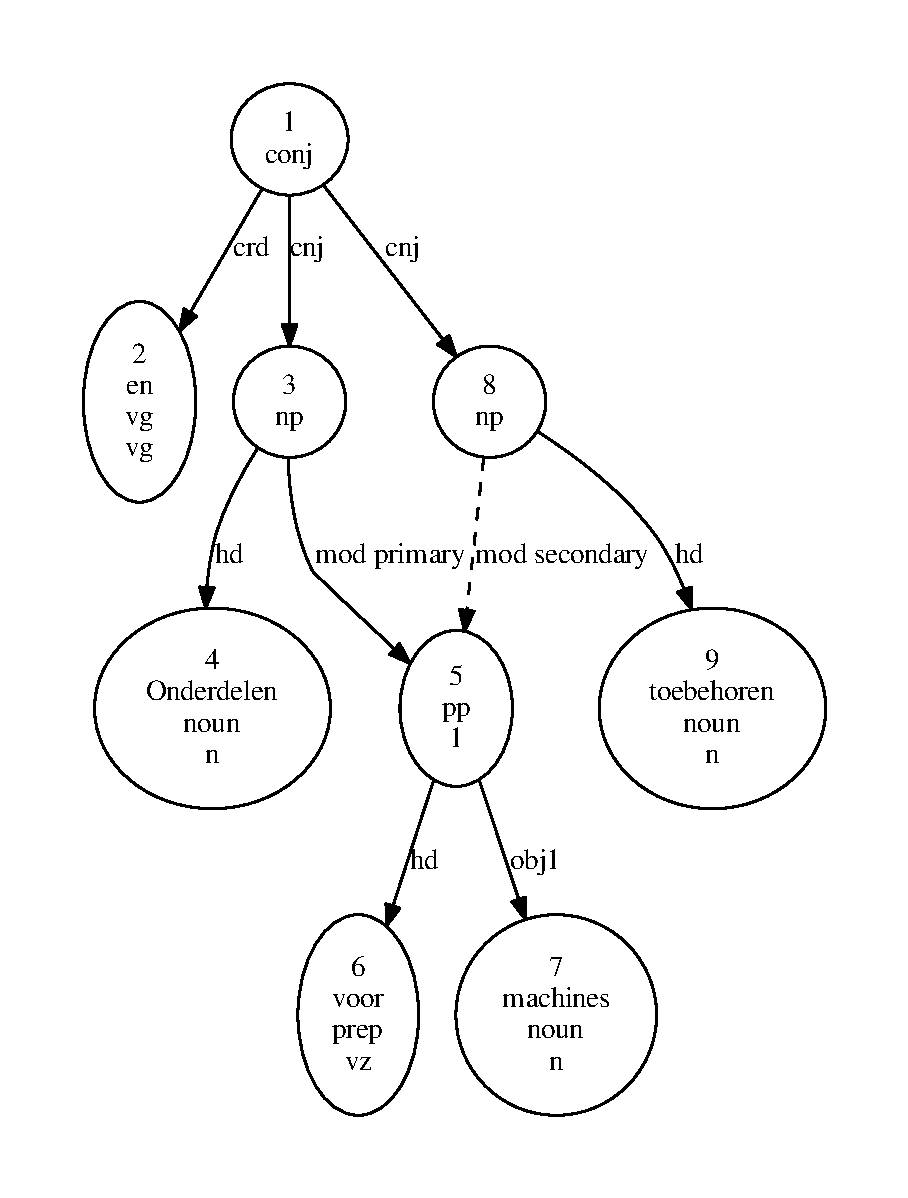
\includegraphics[scale=0.46]{Figures/cnj_mod1.pdf}
        \caption{Before reattachment}
    \end{subfigure}
    \begin{subfigure}[t]{0.49\textwidth}
        \centering
        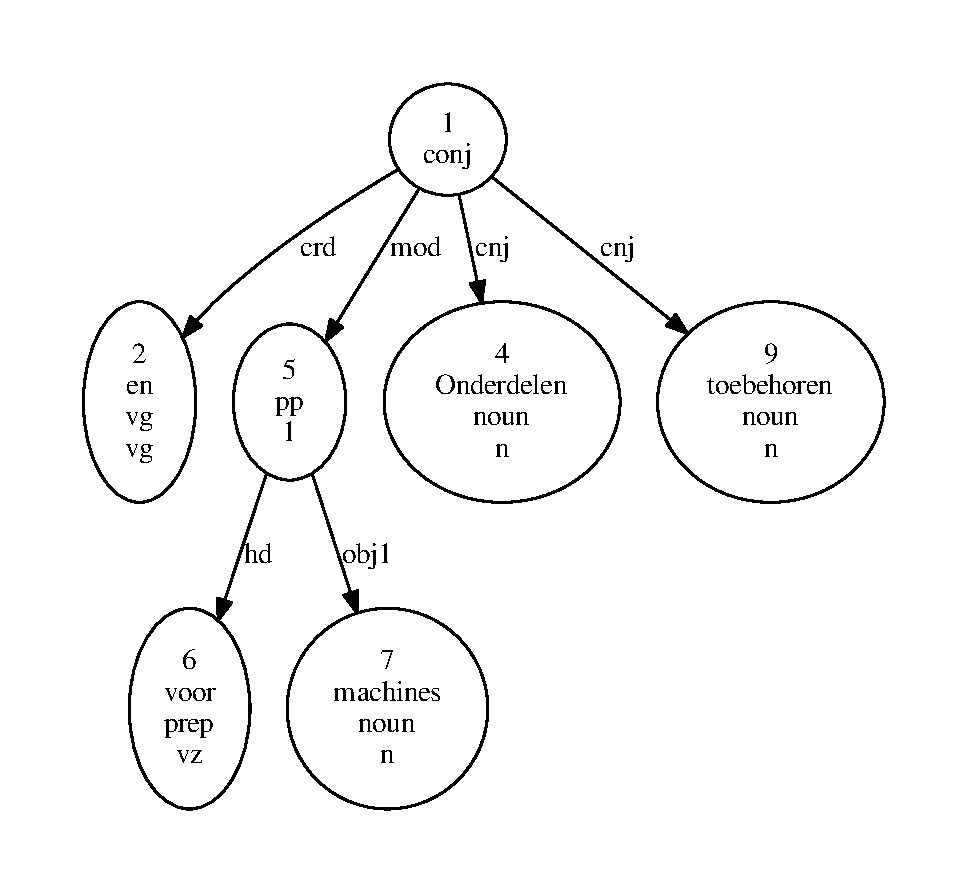
\includegraphics[scale=0.46]{Figures/cnj_mod2.pdf}
        \caption{After reattachment}
    \end{subfigure}
    \caption[Conjunction Modifier Reattachment]{Derivation structure before (a) and after (b) reattachment of shared modifiers for the conjunction ``onderdelen en toebehoren voor machines'' (\textit{parts and accessories for machines}). The transformation detaches the prepositional phrase ``voor machines'' from the two conjuncts it modifies, and connects it once as a daughter of the conjunction node.}
\end{figure}

\subparagraph{Argument Copying} 
If a non-modifying argument is applied on more than one descendants of a conjunction, the type inference process gets slightly more involved.
A minimal solution would be to simply allow copying of the missing material via a unary operator such as ILL's \textit{bang} (!).
Although this trivializes the extraction, it significantly increases the grammar's complexity.
The alternative we pursue instead seeks to perform the type inference process at a local level, deriving the conjunct's type as the result of a partial argument application.
The head functor is allowed to consume its sisters' types, minus the ones that are shared across the conjunction.
The incomplete result, a shorter functor, is used to update the local conjunct's type in a reverse-recursive manner.
The updated conjuncts are then used as the instantiating type for the polymorphic scheme used by the coordinator.
After the coordinator has been applied to all daughters, the remainder is a single instance of this partially reduced functor, which is then allowed to consume the shared arguments.

\subparagraph{Head Copying}
Another common pattern is head copying, where each conjunct has its own individual arguments, but shares the head with its sisters.
Again, a bang operator on the functor would resolve this trivially.
Aside from that, ILL provides another direct solution in virtue of the tensor ($\otimes$); a pair of argument sequences could be converted into a sequence of pairs, to be then consumed by the functor.
Rather than enhancing the logic with the pair type and altering the functor type, we may instead utilize an equivalent implicational type.
That is:
\[
A_1, A_N \vdash (A_1 \rightarrow \dots \rightarrow A_N \rightarrow C) \rightarrow C
\]
which states that from a sequence of assumptions $A_1$,\dots $A_N$, one can derive a higher-order function that accepts a curried function from the sequence to $\Gamma$ to produce a $\Gamma$.
This higher-order proposition at the right hand side of the turnstile is now the instantiating type for the polymorphic coordinator.

To drive the point across, Figure~\ref{fig:head_crd} presents an abstract derivation, with shorthands $Y \equiv A \rightarrow B \rightarrow C$ and $X \equiv Y \rightarrow C$.
A concrete example of the symbolic scheme would be a sentence such as ``logicians like proofs and linguists derivations'', with type assignments: 
\[
\begin{array}{cc}
\text{Word} & \text{Type} \\
\hline
\text{logicians} & A \equiv \textsc{np} \\
\text{proofs} & B \equiv \textsc{np} \\
\text{linguists} & A \\
\text{derivations} & B \\
\text{like} & \quad Y \equiv \textsc{np}\myrightarrow{su}\textsc{np}\myrightarrow{obj1}\textsc{s}_\text{main} \\
\text{and} & \quad \star(Y\rightarrow \textsc{s}_\text{main})\myrightarrow{cnj}Y\rightarrow \textsc{s}_\text{main}

\end{array}
\]


\begin{figure}
    \centering
    \scriptsize
    \[
    \infer[\rightarrow E]{A, Y, B, \star X \rightarrow X, A, B \vdash C}
    {
       \infer[id]{Y \vdash Y}{}
       &
       \infer[\rightarrow E]{A, B, \star X \rightarrow X, A, B \vdash Y \rightarrow C}{
            \infer[\rightarrow I]{A, B \vdash Y \rightarrow C}{
                \infer[\rightarrow E]{A, B, A \rightarrow B \rightarrow C \vdash C}{\dots}
            }
            &
            \infer[\rightarrow E]{A, B, \star X \rightarrow X \vdash X \rightarrow X}{
                \infer[\rightarrow I]{A, B \vdash Y \rightarrow C}{
                    \infer[\rightarrow E]{A, B, A \rightarrow B \rightarrow C \vdash C}{\dots}
                }
                &
                \infer[id]{\star X \rightarrow X \vdash X \rightarrow X \rightarrow X}{}
            }
       }
    }
    \]
    \caption[Head Coordination Schema]{Abstract schema for the derivation of a sentence under head coordination.}
    \label{fig:head_crd}
\end{figure}

\subparagraph{Mixture} 
The last kind of ellipses we need to consider are those where both the head and one or more arguments are shared across the conjuncts, as in the case of a shared phrasal verb.
The treatment is essentially a combination of the two prior cases. 
The type schema remains identical to the simple head coordination, except for the fact that the argument sequence $A_1$,\dots $A_N$ now consists only of the arguments that are uniquely instantiated per daughter, and $\Gamma$ is no longer a simple type, but rather a function type from the common arguments to the conjunction type, as in the simple argument sharing case.

\subparagraph{Non-Polymorphic Ellipses}
Non-polymorphic ellipses occur when there is shared material between two or more conjuncts, but their internal structure does not match, thus rendering our designed solutions unusable.
In total, 400 such annotations occur over the corpus; they are either annotation discrepancies or edge cases necessitating unique modeling. 
A temporary solution is in the works, inspired by ILL's \textit{with} connective (\&).
Its applicability and utility can be evaluated only after a manual inspection of each of these cases, and a correction of those that are indeed erroneous, and is left as future work.

\paragraph{Single Daughter Non-Terminals}
The displacements and detachments performed by the transformations described often result in non-terminal nodes with a single daughter. As the nodes may potentially carry different category tags to their daughters (by-product of some now obsolete phrasal promotion), this can result in inconsistencies among identical or very similar structures. To void this, we collapse non-terminal nodes with a single outgoing edge in an iterative, bottom-up manner, with the resulting node inherits its attributes from its immediate descendant.

\section{Implementation Notes}
Although a full technical overview of the extraction escapes the purposes of this document, this section seeks to provide some key insights on the implementation, in order to make future use and modification easier for any interested party.
The implementation language is Python 3.6; although this choice comes at a cost in elegance compared to a typed language that would naturally accommodate the type system, it is driven by the need for homogeneity and compatibility with the extraction's output's later uses, which will involve statistical learning, for which Python is adopted as the go-to choice.
The extensive number of cases requiring unique treatment demand an iterative approach to the problem, with code parts altered and added as the need arises.
This constantly evolving nature of the codebase makes it hard to design a static software structure that is guaranteed to capture any future grammar alteration or unforeseen edge case.
As such, this section is more of a snapshot of the design at the time of the writing and its overall principles rather than a conclusive technical report.
The extraction code is publicly available at \url{https://github.com/konstantinosKokos/Lassy-TLG-Extraction} and the latest commit at the time of writing is 3d10be8646dfa08d7ead9589297bc264ddd298bb.

\paragraph{System Decomposition}
On the most abstract level, the extraction algorithm may be viewed as a parameterizable map that accepts as input a DAG representing the derivation of a sentence in Alpino-style format as its input, applies a number of modifications on it producing one or more DAGs as an intermediate step, which are then decorated with a type for each of their nodes and returned as the output.

The system consists of two core, interdependent components --- the type component and the extraction component, each enclosed within a corresponding file.
The first implements the particulars of the extracted type system; it defines the classes that implement the type variations present in the grammar, their inductive construction and their means of interaction. 
The second revolves around the treebank transformations and the extraction algorithm itself, as well as providing a wrapper for managing a dataset (i.e. a collection of samples) and a minimal visualization tool.

\subsection{Type System}
The type system is implemented by a hierarchy of classes, each class corresponding to a family of types exhibiting common structure.

\paragraph{WordType} The top class is \textit{WordType}, an abstract class inherited by all other classes which defines the minimal attributes and functions that all other classes must implement.
A listing of class functions shared between all types is given below.
The first is \textit{equality}, a binary function that compares two types based on both their structure and the singular elements they are composed of and returns True if they are in agreement, or False otherwise.
Equality is implemented as a non-commutative function; a type $\textsc{t}_1$ might be left-equal to a type $\textsc{t}_2$ if the latter is a subclass of the former with identical common attributes, but this does not imply the inverse.
The second is \textit{order}, a function that returns a non-negative integer expressing the order of the functor that a type represents.
\textit{Hashing} is a utility function that uniquely maps types to integers, allowing the arrangement of types into sets and dictionaries.
Finally, \textit{string} is a utility function that converts types into a unique and visually informative string format that allows types to be directly printed.

\paragraph{AtomicType}
The simplest class of types and the building block for all other types is \textit{AtomicType}.
These are zero-ary functors, i.e. constants, identified by the strings they were constructed from.
The set of AtomicTypes is provided by the co-domain of the type lexicon, which is a user-specified, many-to-one mapping from part-of-speech tags and phrasal categories to Atomic Types, as seen in Table~\ref{table:lex}.

\paragraph{ComplexType}
The \textit{ComplexType} class implements the family of inductively defined functor types $\textsc{t}_\text{A} \to \textsc{t}_\text{B}$, a unary functor from the argument type $\textsc{t}_\text{A}$ into the result type $\textsc{t}_\text{B}$.
Multi-argument functors are folded into their unary representations; that is, a functor from a sequence of arguments $\textsc{a}_1, \dots \textsc{a}_N$ into a result type $\textsc{r}$ may be written as the $\textsc{a}_1 \to \textsc{a}_2 \to \dots \textsc{r}$, where the ordering can be specified by a preference scheme.
Otherwise, commutativity may be re-introduced by overloading the comparison operator, allowing for an equivalence relation between multi-argument functors to be easily established (useful in cases where no argument ordering is forced).

\paragraph{ColoredType}
\textit{ColoredType} inherits \textit{ComplexType} and implements the family of functor types $\textsc{t}_\text{A} \myrightarrow{c} \textsc{t}_\text{B}$, where $\myrightarrow{c}$ is a subtyped variant of the implication arrow (a ``colored'' arrow), identified by the label c.
Colored types refine the notion of function and allow distinguishing between functors that share the same arguments and result but differ in the means of conversion from the argument space to the result space.
Colors are strings, elements of a closed set defined by a mapping from the dependency relations present in the corpus, as seen in Table~\ref{table:colors}.
Similarly to complex types, multi-argument functors can be restructured into their chained unary counterparts.
In this case, an extra opportunity for binarization arises, as the ordering can be informed by the implication labels rather than the argument types, as described in~\ref{subsec:extraction_alg}.

\paragraph{ModalType}
The \textit{ModalType} class implements a special family of types which are decorated with some unary operator $[.]$.
The class lacks a universal semantics interpretation; they are instead defined on a per-instance basis.
An example of this is the \textit{StarType}, a case of \textit{ModalType} where the operator in question is the $\star$, denoting a sequence of at least 2 repetitions of the argument type.
Other usecases could involve intuitionistic (i.e. non-linear) types, or expanding the grammar with structural control modalities for limiting the application of copying/erasing, exchange and associativity.

\paragraph{Other Types}
A few extra classes of types are implemented, which are not yet used by the extraction process.
They are mentioned here for the sake of completeness, and to showcase how drastic alterations to the extraction may potentially be achieved with only minor changes in the code.

\begin{itemize}
    \item \textbf{DirectedComplexType} \\
    Inherits \textit{ComplexType}, but also includes an implication direction, allowing for the construction of implicational types more akin to the Lambek Calculus.
    \item \textbf{DirectedColoredType}
    Inherits both \textit{DirectedComplexType} and \textit{ColoredType}. Can be used to create types that are simultaneously direction- and dependency-aware.
\end{itemize}

\paragraph{Type Transformations}
The hierarchical arrangement of type-implementing classes is of major practical importance. 
Any subclass of types may be trivially transformed to any higher subclass by simple erasure of the extra information.
Essentially, as long as this design principle is respected, the extraction algorithm and the type system may be further expanded upon, producing more sophisticated type structures while still allowing an immediate interpretation into a less refined variant.
In other words, given an extracted grammar, simpler versions of it can be obtained trivially with neither a do-over of the extraction code or even a repeated run of the algorithm over the corpus.

The inverse process, i.e. refining the extraction, is also largely simplified; one could always simply overload the type constructors being called throughout the DAG iteration, adding any extra required arguments, thus adapting the extracted grammar with only minimal changes over the type inference algorithm.

\subsection{Processing}
As mentioned earlier, the development process of the extraction component had to follow an iterative approach that incorporated solutions for particular cases in a gradual fashion, either as exceptions or general rules and transformations depending on their regularity.
Even though this poses a difficulty in pre-defining a concrete, end-to-end design pattern, extra effort was put into the adaptability and extensibility of the code in order to accommodate future additions and changes.
To that end, the extraction component relies on a simple but robust procedure; a decomposition module that accepts an input sample, applies a series of transformations onto it, and finally calling the type inference algorithm on the result.

This yields a number of significant benefits.
First off, the overall transformation is malleable, being the composition of arbitrary independent functions.
Each transformation is designed individually; as long as its output is compatible with the expected input of another, the two may be seamlessly composed with no added complexity required to model their interaction.
New transformations may be inserted, and existing ones removed or altered, adapting the input DAG to the extraction's needs while keeping the type inference algorithm unchanged.
More practically, as the first transformation is the one responsible of converting the input file into an extraction-compatible format, replacing it with another could admit processing of different input structures.
At the same time, if a new grammar is specified, it suffices to change the last transformation, it being the inference algorithm, virtually allowing switching between implemented grammars at a whim.
Additional post-processing steps may be chained after the inference to convert the type-annotated DAGs into MILL proofs, pairs of word and type sequences, or simply lexicons mapping words to empirical distributions over types. 

Further, the overall process is stateless, letting us capitalize on the independence of a sample's output from inputs other than the current one. 
As such, the extraction lends itself nicely to the MapReduce paradigm~\cite{dean2008mapreduce}, enabling the use of tunable multi-threading and parallel I/O processing.
By performing the corpus transformations dynamically on the input data, rather than sequentially processing and storing intermediate results, storage and processing overhead is minimized. 
The per-sample processing scheme, in combination with lazy evaluation and on-demand reading ensures smooth scaling to arbitrarily large datasets, allowing a perfectly seamless transition to Lassy-Large.

Finally, the extraction boasts minimal system requirements but near-perfect utilization of additional computational resources, despite its complex nature; the whole of Lassy-Small can fully processed in under 2 minutes using a commercial grade computer.

\section{Conclusion}
This section presented the means through which our type-logical grammar, as specified in Chapter~\ref{chapter:tlg}, can be experimentally aligned with real-world data via the means of an extraction algorithm.
We reviewed the algorithm that accomplishes this alignment, the difficulties that may arise in such a process and the transformations required to adopt Lassy's dependency annotations into grammar-compatible structures.
The resulting treebank combines the high-quality of the Lassy-Small with a highly refined type-system, and offers itself for many practical and theoretical applications, ranging from supertagging and constituency parsing to semantic analysis and statistical models of the language as a whole.
It is our hope that as the extraction gets further refined, its output will arise as a useful, publicly available linguistic resource that can act as the groundwork for further research endeavours.